\immediate\write18{makeindex main.nlo -s nomencl.ist -o main.nls}
\documentclass[12pt,a4paper]{report}
\usepackage[utf8]{inputenc}
\usepackage{vietnam}
\usepackage[left=3cm, right=2.2cm, top=2.5cm, bottom=2.5cm]{geometry}
\usepackage{amsmath}
\usepackage{float}
\usepackage{amssymb} 
\usepackage{graphicx} 
\usepackage[hidelinks, unicode]{hyperref}
\usepackage[labelsep=period]{caption}
\usepackage[table]{xcolor}
\usepackage{titletoc}
\usepackage{etoc}
\usepackage{mathptmx}
\usepackage{sectsty}
\usepackage{multirow}
\usepackage{booktabs, tabularx}
\usepackage{courier}
\usepackage{subfig}
\usepackage{nomencl}
\usepackage{titlesec}
\usepackage{enumitem}
\usepackage{anyfontsize}
\usepackage[fontsize=13pt]{scrextend}
\newcommand{\code}[1]{\texttt{#1}}
\renewcommand{\baselinestretch}{1.5}
\renewcommand{\nomname}{Danh mục ký hiệu và viết tắt}


\makenomenclature
\makeatletter
\titlecontents{chapter}[3cm] % <-- seems to set some specific left margin
{\color{black}\bfseries\addvspace{3mm}}
{\makebox[0cm][r]{\MakeUppercase\@chapapp\hspace{.5em}\thecontentslabel\hspace{0.75cm}}}
{} %     ^^^ pretendously zero width box puts its contents in the left margin
{\hfill\makebox[-2cm]{\thecontentspage}}  % 3cm = twice 1.5cm
\chapternumberfont{\Large}
\chaptertitlefont{\Large}

\titleformat{\chapter}[hang] 
{\normalfont\fontsize{14}{15}\bfseries}{CHƯƠNG \thechapter.}{1em}{} 
\titlespacing*{\chapter}{0pt}{-7pt}{7pt}

\titleformat{\section}
{\normalfont\fontsize{13}{15}\bfseries}{\thesection.}{1em}{}
\titlespacing*{\section}{0pt}{-5pt}{-6pt}  

\titleformat{\subsection}
{\normalfont\fontsize{13}{15}\bfseries\itshape}{\thesubsection.}{1em}{}
\titlespacing*{\subsection}{0pt}{-20pt}{-6pt}

\titleformat{\subsubsection}
{\normalfont\fontsize{13}{15}\itshape}{\thesubsubsection.}{1em}{}
\titlespacing*{\subsubsection}{0pt}{-20pt}{-6pt}


\newcommand{\subsubsubsection}[1]{\paragraph{#1}\mbox{}\\}


\setlist[itemize]{itemsep=-0.3em, topsep=0pt}
\setlength\parindent{0pt}
\setlength{\parskip}{10pt}
\setcounter{secnumdepth}{4}
\setcounter{tocdepth}{4}
\geometry{letterpaper}

% \title{\textbf{ĐỒ ÁN CÔNG NGHỆ MỎ}}
% \author{Bùi Trọng Nghĩa\\Diệp Công Trứ}

\begin{document}
\pagenumbering{gobble}
% \thispagestyle{empty}
\clearpage

\pdfbookmark{\contentsname}{content}
% \maketitle

\begin{center}
	\centering
	\text{ĐỒ ÁN ĐƯỢC HOÀN THÀNH TẠI}\\ 
	\textbf{TRƯỜNG ĐẠI HỌC DẦU KHÍ VIỆT NAM}
\end{center}
Người hướng dẫn chính:..................................................\\
(\textit{Ghi rõ họ, tên, học hàm, học vị})\\
\newline
Người hướng dẫn phụ (\textit{Nếu có}):......................................\\
(\textit{Ghi rõ họ, tên, học hàm, học vị})\\
\newline
Người chấm phản biện:....................................................\\
(\textit{Ghi rõ họ, tên, học hàm, học vị})\\
\newline
\newline
\newline
\newline
\newline
\newline
Đồ án được bảo vệ tại:
\begin{center}
	\centering
	\textbf{HỘI ĐỒNG CHẤM ĐỒ ÁN MÔN HỌC}\\
	\textbf{TRƯỜNG ĐẠI HỌC DẦU KHÍ VIỆT NAM}\\
	Ngày .... tháng .... năm ....
\end{center}
\newpage

\begingroup
\fontsize{10pt}{12pt}\selectfont
TRƯỜNG ĐẠI HỌC DẦU KHÍ VIỆT NAM \hspace*{1.5cm} \textbf{CỘNG HÒA XÃ HỘI CHỦ NGHĨA VIỆT NAM}\\
\hspace*{1.7cm}\underline{\textbf{KHOA DẦU KHÍ}} \hspace*{4.4cm} \underline{\textbf{Độc Lập - Tự Do - Hạnh Phúc}}
\endgroup

\begin{center}
	\centering
	\textbf{NHIỆM VỤ ĐỒ ÁN MÔN HỌC}
\end{center}

\textbf{Họ và Tên sinh viên thực hiện:}
	\begin{itemize}
		\item Bùi Trọng Nghĩa - MSSV: 04PET110011
		\item Diệp Công Trứ - MSSV: 04PET110017
	\end{itemize}
\textbf{Ngành:} Khoan - Khai thác dầu khí. \hspace*{3cm}\textbf{Lớp:} K4KKT\\
\textbf{1. Tên đồ án môn học:} Tối ưu hóa khai thác cho giếng dầu bằng phương pháp phân tích điểm nút.\\
\textbf{2. Nhiệm vụ:} \\
\hspace*{1cm}- Tìm hiểu về phương pháp phân tích điểm nút\\
\hspace*{1cm}- Các phương trình đặc tính giếng\\
\hspace*{1cm}- Ứng xử của dòng chảy trong ống\\
\hspace*{1cm}- Tối ưu hóa khai thác cho một giếng dầu\\
\hspace*{1cm}- Xây dựng mô hình phân tích điểm nút để thực hiện tối ưu hóa khai thác cho giếng X.\\
\textbf{3. Ngày giao Đồ án môn học: }20/09/2018\\
\textbf{4. Ngày hoàn thành Đồ án môn học: }17/12/2018\\
\textbf{5. Người hướng dẫn: }
	\begin{itemize}
		\item ThS. Nguyễn Viết Khôi Nguyên
		\item ThS. Phạm Hữu Tài
	\end{itemize}
\begin{flushright}
Bà Rịa - Vũng Tàu, ngày \ldots tháng \ldots năm \ldots
\end{flushright}
\begingroup
\fontsize{12pt}{12pt}\selectfont
\textbf{HIỆU TRƯỞNG} \hspace{30pt} \textbf{TRƯỞNG PHÒNG ĐÀO TẠO} \hspace{30pt} \textbf{NGƯỜI HƯỚNG DẪN}\\
(Ký, ghi rõ họ tên) \hspace{60pt} (Ký, ghi rõ họ tên) \hspace{80pt} (Ký, ghi rõ họ tên)
\endgroup

\newpage

\begingroup
\fontsize{10pt}{12pt}\selectfont
TRƯỜNG ĐẠI HỌC DẦU KHÍ VIỆT NAM \hspace*{1.5cm} \textbf{CỘNG HÒA XÃ HỘI CHỦ NGHĨA VIỆT NAM}\\
\hspace*{1.7cm}\underline{\textbf{KHOA DẦU KHÍ}} \hspace*{4.4cm} \underline{\textbf{Độc Lập - Tự Do - Hạnh Phúc}}
\endgroup

\begin{center}
	\centering
	\textbf{PHIẾU NHẬN XÉT ĐỒ ÁN MÔN HỌC}\\
	\textbf{(Giáo viên ghi nhận xét của mình, bằng tay, vào phần này)}
\end{center}
\begin{enumerate}
	\item[1.] Về hình thức kết cấu Đồ án:\\.....................................................................................................................................
	\item[2.] Về nội dung: 
	\begin{enumerate}
		\item[2.1] Nhận xét về phần tổng quan tài liệu:
	\end{enumerate}
	\item[] ....................................................................................................................................
	\begin{enumerate}
		\item[2.2] Nhận xét về phương pháp nghiên cứu:
	\end{enumerate}
	\item[] ....................................................................................................................................
	\begin{enumerate}
		\item[2.3] Nhận xét về kết quả đạt được:
	\end{enumerate}
	\item[] ....................................................................................................................................
	\begin{enumerate}
		\item[2.4] Nhận xét phần kết luận:
	\end{enumerate}
	\item[] ....................................................................................................................................
	\begin{enumerate}
		\item[2.5] Những thiếu sót và tồn tại của Đồ án:
	\end{enumerate}
	\item[] ....................................................................................................................................
\end{enumerate}
\textbf{Điểm:}....................................................(Ghi bằng chữ)
\begin{flushright}
Bà Rịa - Vũng Tàu, ngày \ldots tháng \ldots năm \ldots \\
\end{flushright}
\hspace{300pt} \textbf{NGƯỜI HƯỚNG DẪN}\\
\hspace*{316pt} (Ký, ghi rõ họ tên)
\newpage
\pagenumbering{roman}

\begin{center}
	\centering
	\textbf{LỜI CAM KẾT}
	\addcontentsline{toc}{section}{LỜI CAM KẾT}
\end{center}
Chúng tôi xin cam đoan những kết quả nghiên cứu được trình bày trong đồ án này là hoàn toàn trung thực, không vi phạm bất cứ điều gì trong luật sở hữu trí tuệ và pháp luật Việt Nam. Nếu sai, chúng tôi sẽ hoàn toàn chịu trách nhiệm trước pháp luật.\\
\hspace*{250pt} \textbf{ĐẠI DIỆN TÁC GIẢ ĐỒ ÁN}\\
\hspace*{280pt} (Ký, ghi rõ họ tên)
\newline
\newline
\hspace*{282pt} \textit{Bùi Trọng Nghĩa}

\clearpage

\begin{center}
	\centering
	\textbf{LỜI CẢM ƠN}
	\addcontentsline{toc}{section}{LỜI CẢM ƠN}
\end{center}
Với lòng biết ơn sâu sắc nhất, nhóm em xin gửi đến quý Thầy Cô ở khoa Dầu Khí – trường Đại Học Dầu Khí Việt Nam, không những dùng tri thức và tâm huyết của mình để truyền đạt vốn kiến thức quý báu cho chúng em trong suốt thời gian học tập tại trường mà còn tạo điều kiện và luôn ủng hộ nhóm em trong quá trình nghiên cứu hoàn thiện đồ án của nhóm. 

Đồng thời chúng em xin gửi lời cám ơn chân thành đến Thầy \textbf{Nguyễn Viết Khôi Nguyên} và Thầy \textbf{Phạm Hữu Tài} đã đồng ý trở thành người trực tiếp hướng dẫn, đưa ra gợi ý và kịp thời chỉ ra những sai sót cho chúng em trong suốt thời gian hoàn thiện đồ án.

Qua quá trình hoàn thiện đồ án, nhóm đã có nhiều cơ hội với những kiến thức mới đồng thời củng cố và vận dụng những kiến thức chuyên ngành vào thực tế, rèn luyện được kĩ năng nghiên cứu thực tế bổ ích từ Thầy \textbf{Nguyễn Viết Khôi Nguyên} và Thầy \textbf{Phạm Hữu Tài}.

Do quá trình thực hiện đồ án còn gặp nhiều khó khăn nên kết quả hoàn thiện còn nhiều thiếu sót. Kính mong quý Thầy, Cô đóng góp thêm ý kiến để những đồ án tiếp theo nhóm em có thể đạt kết quả tốt hơn và có thể hoàn thiện được bản thân mình hơn.
\begin{flushright}
Nhóm chúng em xin chân thành cảm ơn!
\end{flushright}

\newpage
\begin{center}
	\centering
	\textbf{LỜI MỞ ĐẦU}
\end{center}
Nhu cầu năng lượng luôn luôn là những vấn đề cấp thiết nhất đối với các quốc gia đang phát triển trong đó có Việt Nam. Khai thác dầu thô là một trong những phương án tốt nhất để giải quyết vấn đề này. Để khai thác một cách tối ưu nhất, mang lại lợi nhuận tốt nhất, quá trình tối ưu hóa khai thác cần được ưu tiên xem xét hàng đầu. Một trong những phương pháp đem lại hiệu quả tốt nhất được áp dụng trên thế giới là phương pháp phân tích điểm nút. Đồ án này sẽ trình bày về phương pháp phân tích điểm nút để nâng cao khả năng khai thác tại thềm lục địa Việt Nam. Dựa trên sự phân tích mối quan hệ giữa hiệu suất đường dòng vào (IPR, Inflow Performance Relationship) và đường dòng ra (OPR, Outflow Performance Relationship) để có thể đưa ra lưu lượng khai thác tối ưu nhất. Đồng thời đưa ra những yếu tố ảnh hưởng đến dòng vào và dòng ra như kích thước ống cuộn, kích thước đường dòng, áp suất bình tách. Sử dụng các thông số được tính toán để đưa ra được giải pháp cho toàn mỏ.

\tableofcontents
\addcontentsline{toc}{section}{MỤC LỤC}

\listoffigures
\addcontentsline{toc}{section}{DANH SÁCH HÌNH VẼ}

\listoftables
\addcontentsline{toc}{section}{DANH SÁCH BẢNG BIỂU}

\printnomenclature
\addcontentsline{toc}{section}{DANH MỤC KÝ HIỆU VÀ VIẾT TẮT}

\clearpage
\pagenumbering{arabic}
\newpage

\chapter{PHƯƠNG PHÁP PHÂN TÍCH ĐIỂM NÚT}
\section{Hệ thống khai thác}
Để có thể khai thác, vận chuyển sản phẩm từ vỉa cần phải có một hệ thống khai thác hoàn chỉnh. Một hệ thống khai thác hoàn chỉnh phải có sự liên kết giữa đặc tính vỉa và đặc tính hệ thống đường ống, vì vậy khi thực hiện phân tích toàn bộ hệ thống khai thác được xem như là một đơn vị thống nhất \cite{jansen2004modelling}.

Chức năng chính của hệ thống khai thác \cite{haole2003applyreservoir}:
	\begin{itemize}
		\item Cung cấp đường dẫn cho chất lưu từ vỉa lên bề mặt, hoặc đôi khi là từ bề mặt xuống giếng
		\item Tách sản phẩm khai thác thành các thành phần riêng biệt (dầu, khí, nước...)
		\item Giảm thiểu tối đa tác động của những thành phần phụ
		\item Dự trữ sản phẩm
		\item Kiểm soát quá trình khai thác
		\item Cung cấp năng lượng khi năng lượng vỉa suy giảm
		\item Thực hiện khai thác nhân tạo.
	\end{itemize}

Về cơ bản, hệ thống khai thác được chia thành hai hệ thống nhỏ hơn là hệ thống lòng giếng (Hình \ref{fig:well_facilities_system}) và hệ thống bề mặt (Hình \ref{fig:surface_facilities_system}).

Cụ thể những thành phần cơ bản của hệ thống khai thác bao gồm:
	\begin{itemize}
		\item Vùng cận đáy giếng của vỉa
		\item Thân giếng từ vỉa đến đầu giếng
		\item Đường ống dẫn dầu
		\item Các thiết bị bề mặt như bình tách, máy bơm, máy nén, bể chứa...
	\end{itemize}
	\begin{figure}[h]
		\centering
		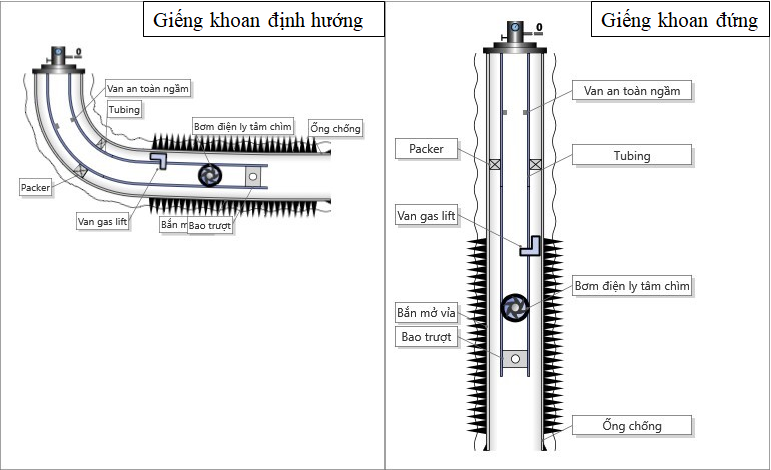
\includegraphics[scale=0.8]{Fig/well_facilities_system.png}
		\caption{Hệ thống lòng giếng}
		\label{fig:well_facilities_system}
	\end{figure}
\newpage
Mỗi thành phần của hệ thống có thể được chia ra làm những thành phần nhỏ hơn. Ví dụ, thân giếng có thể bao gồm:
	\begin{itemize}
		\item Hệ thống bắn mở vỉa
		\item Thiết bị kiểm soát cát
		\item Ống khai thác
		\item Packer, van an toàn ngầm, van gas lift
		\item Hệ thống các van điều khiển đầu giếng
		\item Cây thông khai thác.
	\end{itemize}
Ngoài ra, đối với những giếng cấu trúc đặc biệt như giếng hoàn thiện kép hay giếng hoàn thiện thân trần, những loại giếng này có hệ thống khai thác phức tạp hơn, quá trình phân tích cần nhiều điều kiện đầu vào hơn.
	\begin{figure}[h]
		\centering
		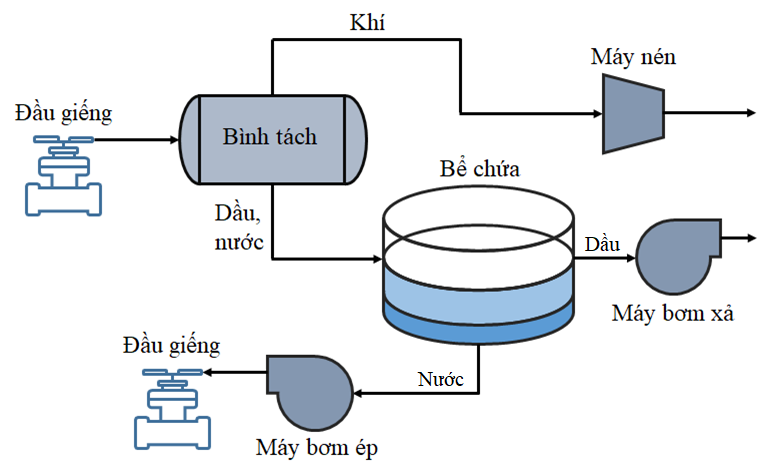
\includegraphics[scale=0.75]{Fig/surface_facilities_system.png}
		\caption{Hệ thống bề mặt}
		\label{fig:surface_facilities_system}
	\end{figure}
\newpage
Đối với hệ thống khai thác khí cần phải có hệ thống xử lý đặc biệt để xử lý các thành phần trong khí khai thác như $\text{CO}_2$, $\text{H}_2\text{S}$ và làm khô khí. Tùy vào mục đích sử dụng mà dòng khí khai thác được có thể được đem bán hoặc bơm ép ngược vào vỉa khi cần. Do đó, hệ thống luôn phải có sẵn các loại máy bơm và máy nén chuyên dụng.

\section{Phân tích điểm nút}

Phương pháp phân tích điểm nút là phương pháp nhằm phân tích ảnh hưởng của các thành phần khác nhau trong một hệ gồm nhiều thành phần như hệ thống mạch điện, mạng lưới đường ống hay bơm ly tâm. Phương pháp phân tích điểm nút được Gilbert ứng dụng lần đầu trong giếng khai thác dầu khí vào năm 1954 và sau đó được Mach, Proano và Brown (1979) phát triển, hiện nay phương pháp phân tích điểm nút trở thành phương pháp không thể thiếu trong việc nghiên cứu thiết kế hệ thống khai thác dầu khí \cite{dale1991production}.

Trong một hệ thống khai thác, tổn thất áp suất xảy ra liên tục khi chất lưu chảy từ vùng dẫn lưu của vỉa qua các thiết bị tới bình tách ở bề mặt (Hình \ref{fig:nodal_system} \cite{dale1991production}). Phương pháp phân tích điểm nút chia hệ thống khai thác thành hai phần bằng một nút với giả thiết rằng lưu lượng vào và ra khỏi một nút là như nhau và ở mỗi một nút chỉ tồn tại một áp suất. Nút có thể được chọn ở các vị trí khác nhau, tuy nhiên thường chọn nhất ở đáy giếng nơi đặt áp kế đo sâu hoặc đầu giếng nơi áp suất có thể đo được bằng áp kế tại cây thông khai thác. Khi đo hoặc tính được áp suất tại mỗi nút, áp suất tổn thất giữa các nút là hàm của lưu lượng, khi đã tìm ra được mối quan hệ giữa lưu lượng và áp suất có thể dùng mô hình để đánh giá tổn thất áp suất ở các lưu lượng khác nhau.
	\begin{figure}[h]
		\centering
		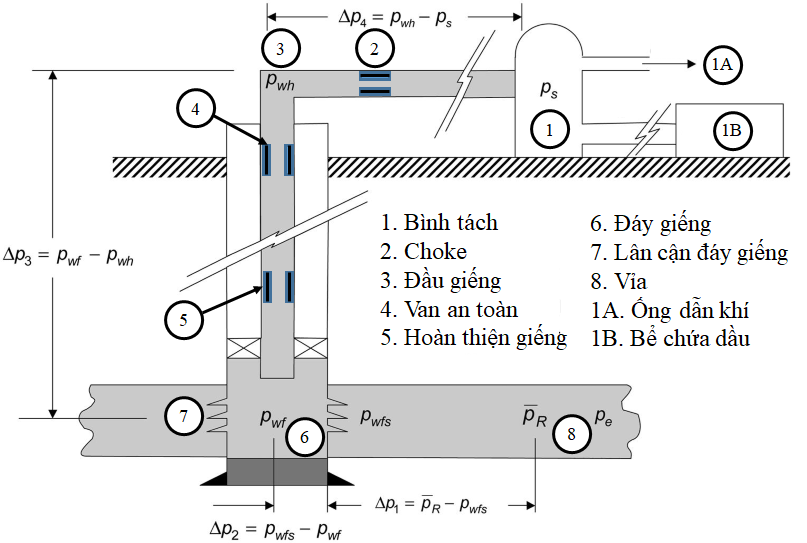
\includegraphics[scale=0.7]{Fig/nodal_system.png}
		\caption{Hệ thống khai thác và các điểm nút thường được chọn}
		\label{fig:nodal_system}
	\end{figure}
\newline
Do tổn thất áp suất ở cả đường dòng vào và cả đường dòng ra đều phụ thuộc lưu lượng, khi dùng một loạt các giá trị lưu lượng khác nhau và tính toán toán giá trị áp suất tại điểm nút tương ứng ta sẽ xây dựng được hai quan hệ là đường dòng vào và đường dòng ra (Hình \ref{fig:operation_point}).

Phương pháp phân tích điểm nút là một phương pháp mạnh dùng để thiết kế bộ thiết bị hoàn thiện giếng và nâng cao hiệu quả khai thác của giếng. Các ứng dụng phổ biến của phương pháp phân tích điểm nút bao gồm:
	\begin{itemize}
		\item Đánh giá lưu lượng;
		\item Lựa chọn đường kính cột ống nâng;
		\item Lựa chọn đường kính hệ thống đường ống;
		\item Lựa chọn áp suất đầu giếng, và kích thước choke bề mặt;
		\item Đánh giá ảnh hưởng của sự suy giảm áp suất vỉa;
		\item Xác định các thành phần cản trở dòng chảy.
	\end{itemize}

Ngoài ra phương pháp phân tích điểm nút có thể được ứng dụng để:
	\begin{itemize}
		\item Lựa chọn kích thước các van bề mặt;
		\item Thiết kế mật độ bắn mở vỉa;
		\item Thiết kế gravel pack;
		\item Thiết kế hệ thống khai thác cơ học;
		\item Tối ưu tỷ số khí lỏng cho hệ thống gaslift;
		\item Đánh giá ảnh hưởng của việc hạ thấp áp suất đầu giếng qua việc sử dụng máy nén;
		\item Đánh giá hiệu quả của các phương pháp kích thích giếng.
	\end{itemize}
Trong phạm vi nghiên cứu của đồ án này, lưu lượng được kiểm soát bằng choke và mô hình phân tích điểm nút sẽ có áp suất đầu vào là áp suất vỉa trung bình, áp suất đầu cuối là áp suất bình tách và nút phân tích được chọn tại đáy giếng. Hệ thống khai thác được chia ra làm 2 phần, đường dòng vào (IPR) \nomenclature{IPR}{Đường đặc tính dòng vào} biểu thị khả năng cho dòng chất lưu từ vỉa vào đáy giếng và đường dòng ra cũng chính là đường dòng lên (VLP) \nomenclature{VLP}{Đường đặc tính dòng lên} biểu thị mối quan hệ giữa lưu lượng và tổn thất áp suất khi chất lưu đi từ đáy giếng đến bình tách.

Áp suất tại nút được tính như sau:

Dòng vào:\nomenclature{$P_{node}$}{Áp suất tại nút}
	\begin{equation}
		P_{node} = P_r - \Delta p_{(front-of-node)}
	\end{equation}
Dòng ra:
	\begin{equation}
		P_{node} = P_{separator} + \Delta p_{(behind-node)}
	\end{equation}
Bản chất của phương pháp phân tích điểm nút là tìm giao điểm của đường dòng vào và dòng ra trên đồ thị lưu lượng, áp suất. Giao điểm này được gọi là điểm làm việc của giếng với tọa độ là lưu lượng làm việc và áp suất đáy giếng tương ứng (Hình \ref{fig:operation_point} \cite{dale1991production}).
	\begin{figure}[h]
		\centering
		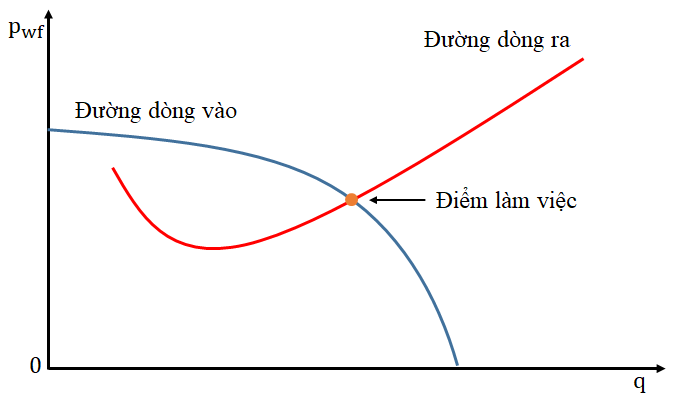
\includegraphics[scale=0.8]{fig/operation_point.png}
		\caption{Điểm làm việc của hệ thống xác định từ đường dòng vào và dòng ra}
		\label{fig:operation_point}
	\end{figure}
\nomenclature{$p_{wf}$}{Áp suất đáy giếng}

\chapter{PHƯƠNG TRÌNH ĐẶC TÍNH}
\section{Định luật Darcy}
Để tính toán sụt áp trong vỉa việc xây dựng phương trình thể hiện tổn thất năng lượng hoặc mất mát áp suất là rất cần thiết. Mặc dù những phương trình này có thể khác nhau tùy thuộc vào loại lưu chất xét đến, tuy nhiên tất cả đều xây dựng dựa trên cơ sở là định luật Darcy.
	\begin{equation}
		v = \dfrac{k}{\mu}\dfrac{dp}{dx}
	\end{equation}
Đối với lưu lượng thể tích q:
	\begin{equation}\label{eqn:2}
		q = vA = -\dfrac{kA}{\mu}\dfrac{dp}{dx}
	\end{equation}
Với:\\
\hspace*{1cm}k: Độ thấm của môi trường rỗng, md\\
\hspace*{1cm}$v$: Vận tốc biểu kiến của lưu chất\\
\hspace*{1cm}q: Lưu lượng thể tích, scf/d\\
\hspace*{1cm}A: Tiết diện dòng chảy, $\text{ft}^2$\\
\hspace*{1cm}$\mu$: Độ nhớt lưu chất, cp\\
\hspace*{1cm}$dp/dx$: Gradient áp suất theo chiều của dòng chảy\\

\subsection{Dòng chảy tuyến tính}
\textit{a. Dòng chảy tầng:}\\
Tổn thất áp suất của dòng chảy tuyến tính qua đường ống có chiều dài L và tiết diện không đổi được thể hiện qua công thức \ref{eqn:1}.
	\begin{equation}\label{eqn:1}
		\int_{p_1}^{p_2}\dfrac{kdp}{\mu} = -\dfrac{q\mu}{kA}\int_o^Ldx
	\end{equation}
Nếu giả sử rằng $k$, $\mu$ và $q$ độc lập với áp suất, phương trình \ref{eqn:1} trở thành:
	\begin{equation}
		p_2-p_1 = -\dfrac{q\mu}{kA}L
	\end{equation}
Hoặc
	\begin{equation}
		q=CkA\dfrac{p_1-p_2}{\mu L}
	\end{equation}
Với:\\
\hspace*{1cm}k: Độ thấm, mD\\
\hspace*{1cm}$\mu$: Độ nhớt, cp\\
\hspace*{1cm}q: Lưu lượng, scf/d\\
\hspace*{1cm}p: Áp suất, psia\\
\hspace*{1cm}L: Chiều dài ống, ft\\
\hspace*{1cm}C: Hệ số chuyển đổi, $C=1$ trong hệ đơn vị Darcy\\
\hspace*{1cm}A: Tiết diện ống, $\text{ft}^2$
	\begin{figure}[h]
		\centering
		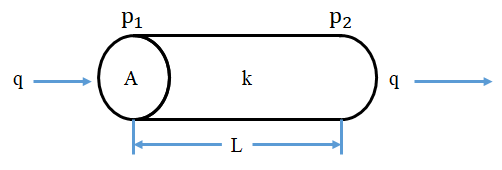
\includegraphics[scale=1]{Fig/darcy_linear_flow.png}
		\caption[Mô hình dòng chảy tuyến tính]{Mô hình dòng chảy tuyến tính \cite{dale1991production}}
		\label{fig:darcy_linear_flow}
	\end{figure}
\newline
\textit{b. Dòng chảy rối:}\\
Đối với dầu:

	\begin{equation}
		p_1-p_2=\dfrac{\mu_oB_oL}{1.127\times 10^{-3}k_oA}q_o
		+\dfrac{9.08\times 10^{-13}B_o^2\beta\rho_oL}{A^2}q_o^2
	\end{equation}
Với:\\
\hspace*{1cm}$p_1$: Áp suất đầu đường ống, psia\\
\hspace*{1cm}$p_2$: Áp suất cuối đường ống, psia\\
\hspace*{1cm}$\mu_o$: Độ nhớt dầu, cp\\
\hspace*{1cm}$B_o$: Hệ số thể tích thành hệ dầu, bbl/STB\\
\hspace*{1cm}L: Chiều dài đường ống, ft\\
\hspace*{1cm}$k_o$: Độ thấm của dầu, md\\
\hspace*{1cm}A: Tiết diện đường ống, $\text{ft}^2$\\
\hspace*{1cm}$\rho_o$: Tỉ trọng của dầu, $\text{lbm}/\text{ft}^3$\\
\hspace*{1cm}$\beta$: Hệ số vận tốc, $\text{ft}^{-1}$\\
\hspace*{1cm}$q_o$: Lưu lượng dầu qua ống, STB/day.

Đối với khí:
	\begin{equation}
		p_1^2-p_2^2=\dfrac{8.93Z\mu_gLT}{k_gA}q_{sc}
		+\dfrac{1.247\times 10^{-16}\beta ZTL\gamma_g}{A^2}q_{sc}^2
	\end{equation}
Với:\\
\hspace*{1cm}Z: Hệ số lệch khí ở nhiệt độ T, áp suất $\overline p$\\
\hspace*{1cm}T: Nhiệt độ, $^o\text{R}$\\
\hspace*{1cm}$\gamma_g$: Tỉ trọng khí\\
\hspace*{1cm}$q_{sc}$: Lưu lượng khí tại 14.7 psia, $60^o\text{F}$, scf/day\\
\hspace*{1cm}$\mu_g$: Độ nhớt khí tại $\overline T$, $\overline p$, cp\\
\hspace*{1cm}$k_g$: Độ thấm đối với khí, md\\
\hspace*{1cm}$\beta$: Hệ số vận tốc, $\text{ft}^{-1}$\\
\hspace*{1cm}$A$: Tiết diện đường dòng, $\text{ft}^2$\\

\subsection{Dòng chảy hướng tâm}

Khi dòng chảy bắt đầu chảy vào giếng sẽ chuyển dần sang dòng chảy hướng tâm. Lúc này tiết diện dòng chảy trở thành một biến số, tuy nhiên vẫn có thểm áp dụng định luật Darcy cho trường hợp này\cite{dale1991production}.

Biến đổi phương trình \ref{eqn:2} theo đạo hàm áp suất với bán kính ảnh hưởng của giếng ta được:
	\begin{equation}
		q = \dfrac{2\pi rhk dp}{\mu dr}
	\end{equation}
Mô hình dòng chảy hướng tâm được thể hiện trong Hình \ref{fig:darcy_radial_flow} \cite{dale1991production}:
	\begin{figure}[h]
		\centering
		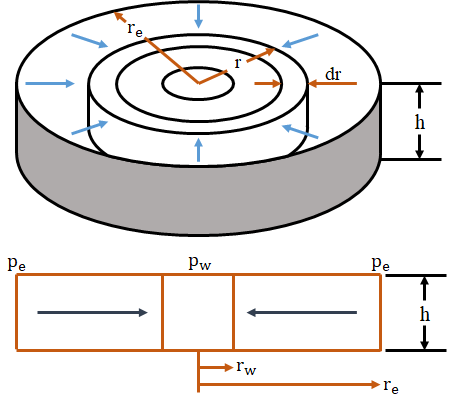
\includegraphics[scale=0.75]{Fig/darcy_radial_flow.png}
		\caption{Mô hình dòng chảy hướng tâm}
		\label{fig:darcy_radial_flow}
	\end{figure}
\newpage
Đối với dầu:

Dầu được giả sử là lưu chất có tính nén yếu, tính nén này được thể hiện thông qua hệ số thể tích thành hệ dầu, vì vậy lưu lượng dầu vẫn được tính toán ở điều kiện bề mặt.
	\begin{equation}\label{eqn:3}
		q_oB_o=\dfrac{2\pi rhk_o}{\mu_o}\left(\dfrac{dp}{dr}\right)
	\end{equation}
Nếu như dòng chảy trong vỉa là dòng chảy ổn định hay dòng chảy tầng, đạo hàm áp suất coi như không đổi, đồng thời các đơn vị đo lường cho các đại lượng tính toán là đơn vị mỏ dầu khí (field units), phương trình \ref{eqn:3} trở thành:
	\begin{equation}
		q_o = \dfrac{0.00708k_oh(\overline p-p_{wf})}{\mu_oB_o.ln(0.472r_e/r_w)}
	\end{equation}
Với $\overline p$ là áp suất trung bình của vỉa.

Đối với khí:

Lưu lượng khí được xác định ở điều kiện tiêu chuẩn $p_{sc} = 14.7 psia$, $T_{sc}=520^oR$:
	\begin{equation}
		q_{sc}=\dfrac{703\times 10^{-6}k_gh(\overline p_R^2-p_{wf})}{\mu_gZT.ln(0.472r_e/r_w)}
	\end{equation}

Ứng xử của áp suất vỉa:

Ứng xử của áp suất vỉa được xem như một hàm phụ thuộc vào bán kính ảnh hưởng của giếng.
	\begin{equation}
		p = \overline p_R - \dfrac{141.2q_o\mu_oB_o}{k_oh}ln(0.472r_e)
		+\dfrac{141.2q_o\mu_oB_o}{k_oh}ln(r)
	\end{equation}
Mối quan hệ giữa áp suất vỉa và bán kính ảnh hưởng được thể hiện thông qua đồng thị Hình \ref{fig:p_reservoir_vs_radius} \cite{dale1991production}, cho thấy gradient áp suất tăng nhanh trong vùng chuyển tiếp từ bán kính giếng tới bán kính vỉa.
	\begin{figure}[h]
		\centering
		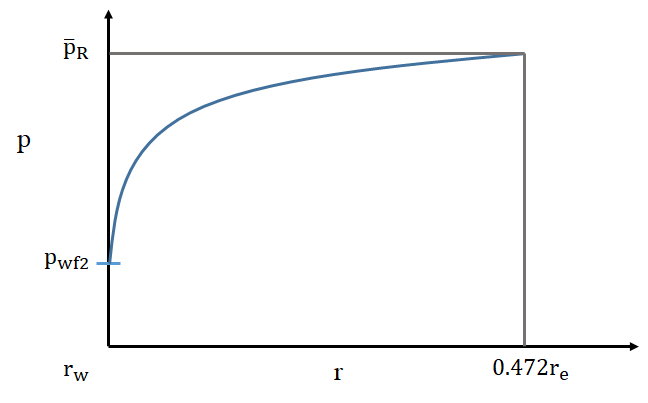
\includegraphics[scale=0.75]{Fig/p_reservoir_vs_radius.png}
		\caption{Ứng xử của áp suất vỉa}
		\label{fig:p_reservoir_vs_radius}
	\end{figure}
\newline
Nếu như đồ thị Hình \ref{fig:p_reservoir_vs_radius} được thể hiện ở dạng \text{semi-log} (Hình \ref{fig:p_reservoir_vs_radius_semi_log} \cite{dale1991production}) mối quan hệ giữa $p$ và $ln(r)$ sẽ trở thành dạng đường thẳng với hệ số góc m. Với m:
	\begin{equation}
		m = \dfrac{141.2q_o\mu_oB_o}{k_oh}
	\end{equation}
Tương tự, hệ số góc m cho dòng chảy của chất khí:
	\begin{equation}
		m = \dfrac{1422q_{sc}\mu_gZT}{k_gh}
	\end{equation}
	\begin{figure}[h]
		\centering
		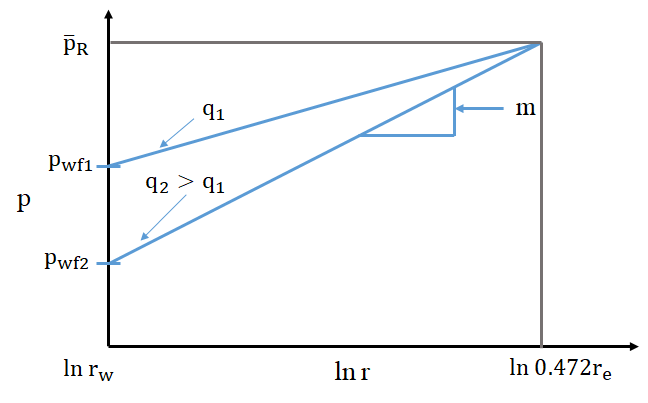
\includegraphics[scale=0.75]{Fig/p_reservoir_vs_radius_semi_log.png}
		\caption{Đồ thị semi-log của áp suất và bán kính ảnh hưởng}
		\label{fig:p_reservoir_vs_radius_semi_log}
	\end{figure}

\section{Chỉ số khai thác}
Mối quan hệ giữa lưu lượng dòng vào và mức độ giảm áp suất thường được thể hiện bằng chỉ số khai thác (\textit{Productivity Index, J}).
	\begin{equation}
		J = \dfrac{0.00708k_oh}{\mu_oB_o.ln(0.472r_e/r_w)}
	\end{equation}
Lưu lượng dòng vào của dầu được thể hiện qua phương trình:
	\begin{equation}
		q_o = J(\overline p_R - p_{wf})
	\end{equation}
Hay:
	\begin{equation}
		J = \dfrac{q_o}{\overline p_R - p_{wf}}
	\end{equation}
Các yếu tố ảnh hưởng đến chỉ số khai thác:
	\begin{itemize}
		\item Ứng xử pha của vỉa
		\item Độ thấm tương đối
		\item Độ nhớt của dầu
		\item Hệ số thể tích thành hệ
	\end{itemize}
\subsection{Ứng xử pha của vỉa}
Giản đồ pha của một vỉa thông thường được thể hiện như trong Hình \ref{fig:phase_behavior_in_pi} \cite{ahmed2006reservoir}.
	\begin{figure}[h]
		\centering
		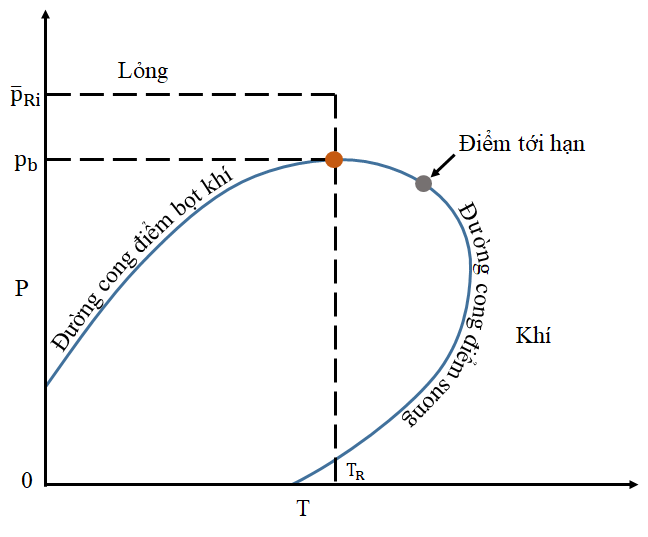
\includegraphics[scale=0.8]{Fig/phase_behavior_in_pi.png}
		\caption{Giản đồ pha của một vỉa thông thường}
		\label{fig:phase_behavior_in_pi}
	\end{figure}
\newline
Khi áp suất vỉa ban đầu lớn hơn áp suất điểm bọt khí, lúc này trong vỉa chưa có sự xuất hiện của khí. Tuy nhiên, khi áp suất vỉa giảm xuống dưới áp suất điểm bọt khí, khí tự do bắt đầu được hình thành dẫn tới sự suy giảm của độ bão hòa dầu tương đối. Khi tiến hành khai thác ở điều kiện áp suất vỉa dưới điểm bọt khí, chỉ số khai thác thường giảm nhanh. Trong thực tế, trường hợp này có thể xảy ra kể cả khi áp suất vỉa lớn hơn áp suất bão hòa \cite{standing1951volumetric}.\\

\subsection{Độ thấm tương đối}
Khi khí tự do hình thành trong vỉa, khả năng cho dòng của pha lỏng trong vỉa giảm. Điều này xảy ra kể cả khi độ bão hòa khí không đủ lớn để tạo thành dòng chảy của khí \cite{dale1991production}. Ứng xử của độ thấm tương đối được thể hiện trong Hình \ref{fig:kro_behavior_pi} \cite{dale1991production}.
	\begin{figure}[h]
		\centering
		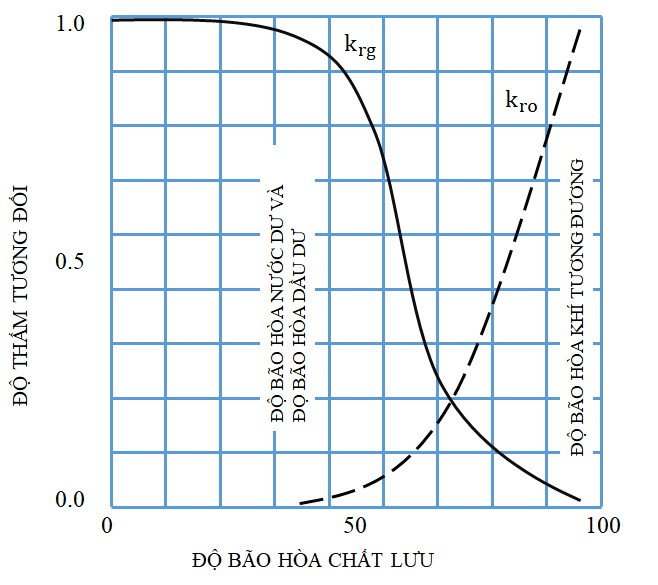
\includegraphics[scale=0.65]{Fig/kro_behavior_pi.png}
		\caption{Ứng xử của độ thấm tương đối}
		\label{fig:kro_behavior_pi}
	\end{figure}

\subsection{Độ nhớt của dầu}
Độ nhớt của dầu bão hòa tại nhiệt độ không đổi giảm khi áp suất vỉa bắt đầu giảm xuống tới áp suất bão hòa. Dưới áp suất bão hòa, độ nhớt của dầu tăng trở lại khi có sự thoát ra của khí hòa tan, làm cho pha lỏng trở nên kém linh động hơn (Hình \ref{fig:oil_viscosity_behavior} \cite{ahmed2006reservoir}).\\

\subsection{Hệ số thể tích thành hệ}
Khi áp suất bắt đầu giảm, lưu chất sẽ giản nở. Khi áp suất vỉa giảm xuống dưới điểm áp suất bão hòa khí bắt đầu thoát ra làm cho dầu co lại (Hình \ref{fig:bo_behaviour_pi} \cite{ahmed2006reservoir}). Hệ số thể tích thành hệ thể hiện độ co ngót lại đó của lưu chất.
	\begin{equation}
		B_o = \dfrac{(V_o+V_{gas-dissolved})_{(p, T)}}{(V_o)_{(p_{sc}, T_{sc})}}
	\end{equation}
\newpage
	\begin{figure}[h]
		\centering
		\subfloat[Độ nhớt\label{fig:oil_viscosity_behavior}]
  			{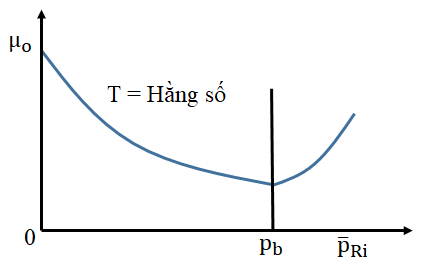
\includegraphics[scale=0.65]{Fig/oil_viscosity_behavior.png}}\hfill
		\subfloat[Hệ số thể tích thành hệ\label{fig:bo_behaviour_pi}]
  			{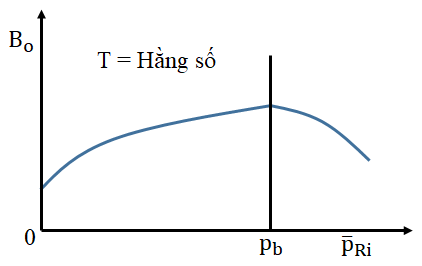
\includegraphics[scale=0.65]{Fig/bo_behaviour_pi.png}}\hfill
		\caption{Ứng xử của độ nhớt dầu và hệ số thể tích thành hệ}
	\end{figure}

\section{Đường đặc tính dòng vào}

Đường đặc tính dòng vào biểu hiện mối quan hệ giữa lưu lượng và áp suất đáy giếng ứng với một áp suất vỉa nhất định. Hình dạng và kích thước đường dòng vào phụ thuộc vào các đặc tính thấm dẫn của đá vỉa và áp suất vỉa.

Theo lý thuyết đường dòng vào, lưu lượng bằng 0 khi áp suất đáy giếng bằng áp suất vỉa. Khi áp suất đáy giếng giảm xuống, chênh lệch áp suất trong vỉa và đáy giếng tăng, thế năng sinh ra đẩy dầu khí đi vào đáy giếng nhiều hơn. Áp suất đáy giếng càng thấp lưu lượng dầu, khí bị đẩy vào giếng càng lớn. AOF (absolute open flow) \nomenclature{AOF}{Dòng mở tuyệt đối} là lưu lượng tối đa đi vào giếng khi áp suất đáy giếng giảm xuống bằng không. Trong thực tế, áp suất đáy giếng không thể giảm xuống tới giá trị này. Tuy nhiên, AOF thường là tiêu chí để đánh giá khả năng cho dòng của giếng và chất lượng của vỉa.

Đường IPR có thể được xây dựng bằng lý thuyết dòng chảy Darcy và tương quan thực nghiệm. Cần đối chiếu với các kết quả thử giếng để đảm bảo đường IPR đã xây dựng phản ánh đúng khả năng cho dòng của vỉa. Đường IPR có hình dạng phụ thuộc vào đặc tính thấm dẫn của vỉa và áp suất vỉa ban đầu. Theo thời gian, khi áp suất vỉa suy giảm hay đặc tính thấm dẫn của vỉa giảm thì đường IPR sẽ dịch chuyển dần về phía gốc tọa độ, biểu thị khả năng cho dòng của vỉa giảm đi.

	\begin{figure}[h]
		\centering
		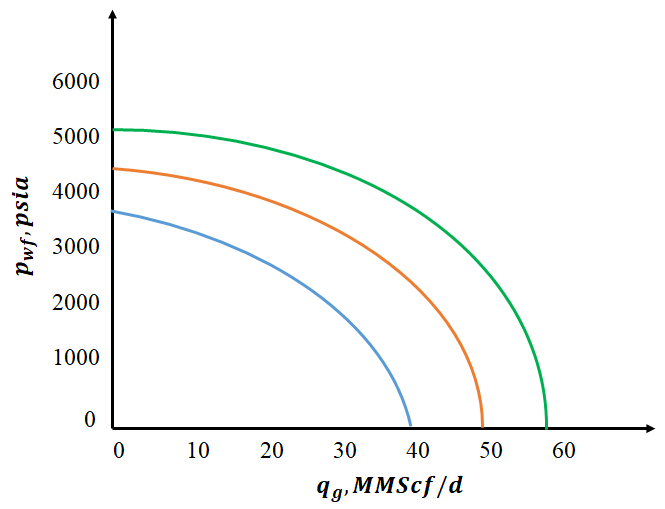
\includegraphics[scale=0.75]{fig/ipr_change_with_pressure.png}
		\caption{Đường IPR thay đổi khi áp suất vỉa suy giảm.}
		\label{fig:ipr_change_with_pressure}
	\end{figure}

\textit{Các yếu tố ảnh hưởng lên đường đặc tính dòng vào}

Đối với một vỉa dầu (khí) đường đặc tính dòng vào thường bị ảnh hưởng trực tiếp bởi những cơ chế sau:
	\begin{itemize}
		\item Sự thay đổi độ thấm tương đối của dầu khi độ bão hòa khí thay đổi
		\item Sự thay đổi độ nhớt của dầu khi áp suất và lượng khí thoát ra thay đổi
		\item Sự thay đổi độ co ngót của dầu đồng thời khí thoát ra khi áp suất giảm
		\item Quá trình hoàn thiện giếng (nhiễm bẩn hay kích thích thành hệ)
		\item Sự thay đổi hệ số bất ổn khi lưu lượng dòng vào tăng.
	\end{itemize}
Những yếu tố này có thể thay đổi khi có sự thay đổi của sụt áp (drawdown).\\

\subsection{Cơ chế năng lượng vỉa}
Nguồn năng lượng của vỉa đưa dầu, khí vào giếng ảnh hưởng đáng kể đến cả đặc tính vỉa và hệ thống khai thác.

\textit{a. Cơ chế khí hòa tan}

Với cơ chế khí hòa tan, khi bắt đầu khai thác áp suất vỉa giảm nhanh đếm điểm áp suất bão hòa. Sau khi giảm xuống dưới điểm áp suất bão hòa khí tự do bắt đầu xuất hiện, áp suất vỉa vẫn tiếp tục giảm nhưng tốc độ chậm hơn đồng thời tỉ lệ khí dầu cũng tăng lên.

Sau một thời gian dài khai thác, lúc này lượng khí tự do bắt đầu giảm do quá trình khai thác. Do đó, tỉ số khí dầu bắt đầu giảm xuống. Thời điểm này các phương pháp nhân tạo sẽ được tiến hành để có thể duy trì áp suất vỉa và kéo dài thời gian khai thác.

Lượng dầu thu hồi được đối với cơ chế này thường vào khoảng 5 - 30 \% lượng dầu ban đầu trong vỉa.

\textit{b. Cơ chế mũ khí}

Với cơ chế mũ khí, áp suất vỉa giảm chậm hơn so với cơ chế khí hòa tan. Dưới những điều kiện cơ bản chưa có sự can thiệp của các phương pháp duy trì áp suất vỉa, lượng dầu thu hồi được thường vào khoảng 20 - 40 \% lượng dầu ban đầu trong vỉa.

\textit{c. Cơ chế tầng nước đáy}

Đối với những vỉa có cơ chế năng lượng này sau khi áp suất vỉa giảm xuống dưới điểm áp suất bão hòa, vỉa sẽ được cung cấp thêm năng lượng từ cơ chế khí hòa tan.

Do khả năng cung cấp năng lượng lâu dài của tầng nước đáy, lượng dầu thu hồi được từ những vỉa này thường cao từ 35 - 75 \% lượng dầu ban đầu trong vỉa.

\textit{d. Cơ chế kết hợp}

Trong nhiều trường hợp, vỉa có thể có cả ba cơ chế năng lượng đã nêu ở trên. Đối với những vỉa này quá trình khai thác thường dễ xảy ra vấn đề do sự giãn nở cùng lúc của tầng nước đáy và khí tự do làm cho mặt tiếp xúc khí-dầu và mặt tiếp xúc dầu-nước gặp nhau.

Khả năng thu hồi dầu của những vỉa này cũng khó có thể được xác định. Điều này còn phụ thuộc vào kích thước của mũ khí và tầng nước đáy. Khi thực hiện khai thác trên những vỉa có cơ chế năng lượng kết hợp, bơm ép khí và bơm ép nước thường được thực hiện để hạn chế vấn đề xảy ra.\\

\subsection{Mức giảm áp và lưu lượng khai thác}

\textit{a. Hệ số nhiễm bẩn bằng không}

Đối với áp suất vỉa lớn hơn áp suất bão hòa, nếu lưu lượng dòng vào có thể đạt được giá trị monh muốn trong khi $p_{wf_1} \geq p_b$ thì giá trị $f(p)$ sẽ là hằng số tại mọi điểm nằm trong vùng bán kính ảnh hưởng của giếng với $J$ không đổi.

Nếu cần phải tăng lưu lượng khai thác lơn hơn so với $q_0$, áp suất vỉa $p_{wf}$ phải tiếp tục giảm. Nếu $p_{wf_2}$ nhỏ hơn so với $p_b$, sự bão hòa khí tự do sẽ xảy ra bên ngoài bán kính ảnh hưởng $r_2$, độ thấm tương đối của dầu giảm trong khi hệ số góc của đường cong áp suất tăng trong vùng bán kính giếng tới bán kính ảnh hưởng $r_2$.
	\begin{figure}[h]
		\centering
		\subfloat[Sự thay đổi áp suất vỉa\label{fig:reservoir_pressure_profile}]
  			{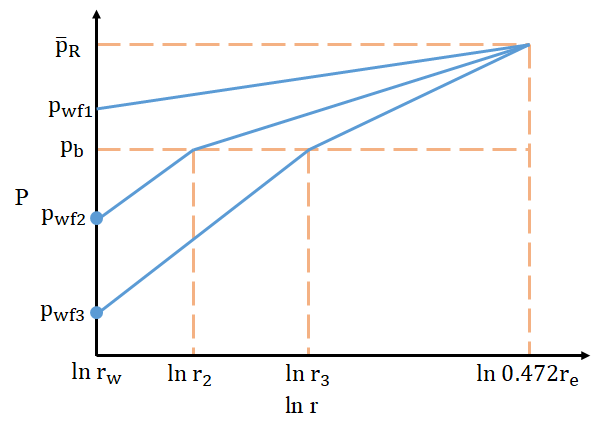
\includegraphics[scale=0.5]{Fig/reservoir_pressure_profile.png}}\hfill
		\subfloat[Đường cong đặc tính dòng vào\label{fig:inflow_performance_relationship}]
  			{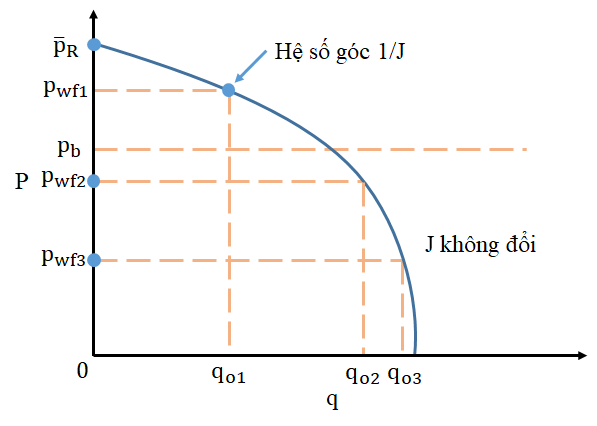
\includegraphics[scale=0.5]{Fig/inflow_performance_relationship.png}}\hfill
		\caption{Độ giảm áp và lưu lượng khai thác}
		\label{fig:reservoir_pressure_relationship}
	\end{figure}
\newpage
Khi áp suất vỉa giảm tới $p_{wf_3}$, độ thấm tương đối của dầu tiếp tục giảm trong bán kính ảnh hưởng $r_3$ và tăng hệ số góc của đường cong đặc tính dòng vào. Chi tiết được thể hiện trong đồ thị Hình \ref{fig:reservoir_pressure_relationship} \cite{dale1991production}.

\textit{b. Hệ số nhiễm bẩn âm hoặc dương}

Hệ số nhiễm bẩn thành hệ khác không chứng tỏ rằng tổn thất áp suất có chứa các thành phần mất mát gây ra bởi nhiễm bẩn thành hệ hay kích thích vỉa. Giếng bị nhiễm bẩn thường gây khó khăn trong quá trình xây dựng đường đặc tính dòng vào.

Với trường hợp giếng bị nhiễm bẩn (S' > 0) \nomenclature{$S, S'$}{Hệ số nhiễm bẩn thành hệ}, sự bảo hòa khí có thể không tồn tại trong vỉa kể cả khi $p_{wf} < p_b$ (Hình \ref{positive_skin_effect} \cite{dale1991production}). Với trường hợp giếng đã được xử lý (S' < 0) tổn thất áp suất có thể được bỏ qua (Hình \ref{fig:negative_skin_effect} \cite{dale1991production}).
	\begin{figure}[h]
		\centering
		\subfloat[Hệ số nhiễm bẩn dương\label{positive_skin_effect}]
			{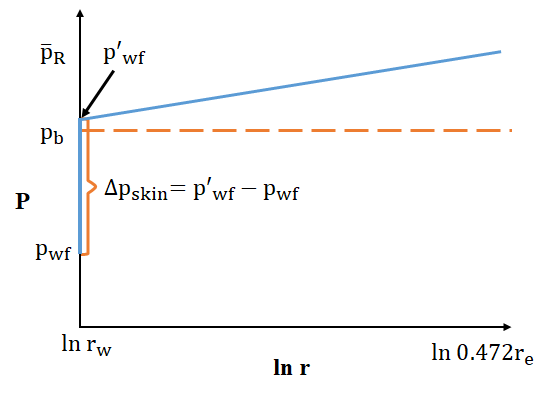
\includegraphics[scale=0.55]{Fig/positive_skin_effect.png}}\hfill
		\subfloat[Hệ số nhiễm bẩn âm\label{fig:negative_skin_effect}]
			{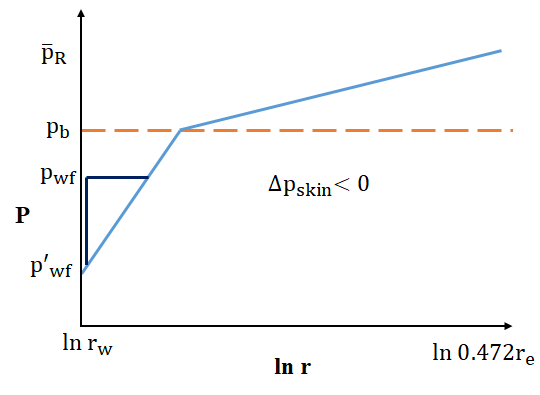
\includegraphics[scale=0.55]{Fig/negative_skin_effect.png}}\hfill
		\caption{Ảnh hưởng của hệ số nhiễm bẩn}
	\end{figure}

\subsection{Suy kiệt năng lượng vỉa}

Ở những vỉa không thể duy trì áp suất vỉa trung bình trên áp suất bão hòa, hiện tượng bão hòa khí tự do sẽ xảy ra ở toàn bộ thể tích tháo cạn (drainage volume) của giếng. Hiện tượng này làm giảm độ thấm tương đối của dầu đồng thời tăng hệ số góc của đường cong áp suất và đường đặc tính dòng vào.

Để có thể duy trì lưu lượng dòng vào không đổi việc tăng độ giảm áp suất (drawdown) tương ứng với áp suất vỉa suy giảm là rất cần thiết.\\

\subsection{Ứng xử của đường đặc tính dòng vào giếng khí}

Đối với giếng khí, lưu lượng dòng vào là một hàm của bình phương áp suất đáy giếng. Vì vậy đường đặc tính dòng vào của giếng khí không có dạng tuyến tính. Trong những vỉa khí khô và khí ướt không có mặt khí ngưng tụ và sự bão hòa khí, độ thấm tương đối của khí luôn không đổi kể cả khi áp suất vỉa trung bình suy giảm. Nếu dòng chảy rối tồn tại, tổn thất áp suất sẽ tăng khi lưu lượng tăng, gây ra sự suy giảm của đường đặc tính dòng vào.

Nếu không có pha lỏng hình thành cho vỉa, sự suy kiệt năng lượng vỉa không phải là nguyên nhân làm cho độ thấm tương đối của khí giảm. Tuy nhiên, sự suy kiệt năng lượng vỉa có thể làm tăng dòng chảy rối do vận tốc thực tế lớn hơn so với cần thiết để duy trì lưu lượng khối không đổi. Đồng thời tích của giá trị $\mu Z$ \nomenclature{$Z$}{Hệ số lệch khí} cũng thay đổi khi áp suất vỉa thay đổi \cite{dale1991production}.

\section{Đường đặc tính dòng lên}

Những thành phần của hệ thống khai thác nằm phía sau điểm nút được chọn (theo hướng dòng từ vỉa đi lên) được gọi là phần dòng ra. Đường cong thể hiện mối quan hệ giữa áp suất dòng ra và lưu lượng chính là đường đặc tính dòng ra (OPR) hay còn gọi là đường đặc tính dòng lên (VLP).

Đường đặc tính dòng lên thể hiện cho khả năng đưa lưu chất từ đáy giếng lên bề mặt với áp suất đầu giếng xác định. Với đường đặc tính dòng lên lưu lượng khai thác của giếng có thể được xác định tại điều kiện vận hành cho trước.

Như đã nêu ở trên, trong phạm vi của đồ án nhóm tác giả chỉ chọn một điểm nút tại đáy giếng. Khi đó, hệ thống dòng ra bao gồm:
	\begin{itemize}
		\item Ống khai thác
		\item Đầu giếng
		\item Choke
		\item Ống dòng
		\item Bình tách.
	\end{itemize}

\section{Ảnh hưởng của hoàn thiện giếng}

Có ba loại hoàn thiện giếng cơ bản dựa trên loại giếng, độ sâu giếng và loại vỉa hoặc thành hệ. Trong một số trường hợp giếng được hoàn thiện thân trần (open hole), hoàn thiện giếng bắn mở vỉa (perforated completion) và hoàn thiện giếng kết hợp bắn mở vỉa với chèn sỏi (perforated, gravel-pack completion).

Để tính toán suy giảm áp suất do hoàn thiện giếng, phương trình dòng vào tổng quát có thể được thay đổi để phù hợp với ảnh hưởng của hoàn thiện giếng và cho mọi loại hoàn thiện. Phương trình cho cả dòng chảy với chất lưu dầu và khí được trình bày như sau:
	
	\begin{equation}\label{eqn:4}
		q_o = \dfrac{0.00708k_oh(\overline p_R-p_{wf})}{\mu_oB_o([ln(0.472r_e/r_w)]+S')}
	\end{equation}
	
	\begin{equation}\label{eqn:5}
		q_{sc}=\dfrac{703\times 10^{-6}k_gh(\overline p_R^2-p_{wf}^2)}{\mu_g\overline ZT[ln(0.472r_e/r_w)]+S'}
	\end{equation}
Với
	\begin{equation}
		S' = S + Dq
	\end{equation}
Giá trị S' có thể đạt được từ thí nghiệm dòng chảy chuyển tiếp một lưu lượng, tuy nhiên để xác định giá trị cho S và D \nomenclature{D}{Hệ số độ rối} yêu cầu thí nghiệm dòng chảy chuyển tiếp với hai lưu lượng khác nhau.

Phương trình \ref{eqn:4} và \ref{eqn:5} có thể được viết trong dạng khác:

	\begin{equation}
		\overline p_R - p_{wf} = Aq_o + Bq_o^2
	\end{equation}
	\begin{equation}
		\overline p_R^2 - p_{wf}^2 = Aq_{sc} + Bq_{sc}^2
	\end{equation}
A là hệ số chảy tầng và B là hệ số chảy rối. Hai hệ số này có thể được xác định từ sự kết hợp của một vài thành phần và dựa vào đặc tính hoàn thiện giếng:
	\begin{equation}
		A = A_R + A_P + A_G
	\end{equation}
	\begin{equation}
		B = B_R + B_P + B_G
	\end{equation}
Trong đó:\\
\hspace*{1cm}$A_R$: thành phần vỉa chảy tầng\\
\hspace*{1cm}$A_P$: thành phần bắn mở vỉa chảy tầng\\
\hspace*{1cm}$A_G$: thành phần gravel-pack chảy tầng\\
\hspace*{1cm}$B_R$: thành phần vỉa chảy rối\\
\hspace*{1cm}$B_P$: thành phần bắn mở vỉa chảy rối\\
\hspace*{1cm}$B_G$: thành phần gravel-pack chảy rối

Những thành phần này có những định nghĩa khác nhau cho dòng chảy dầu và khí, chỉ các giá trị hệ số A và B có thể có được từ test khai thác trong giếng đã được hoàn thiện, vì vậy hàm số để ước tính giá trị của các thành phần phải có sẵn.

\chapter{DÒNG CHẢY TRONG ỐNG}
\section{Thành phần tổn hao áp suất}

Để xác định đặc tính của một giếng khai thác cần phải tính toán tổn hao áp suất của toàn bộ thành phần thiết bị trong hệ thống khai thác. Các thành phần tổn hao áp suất này được thể hiện như trong Hình \ref{fig:nodal_system}.

Đối với một hệ thống khai thác thông thường áp suất đáy giếng được tính như sau:

	\begin{equation}
		p_{wf}=p_{sep}+\Delta p_{fl} +\Delta p_{choke} + \Delta p_{tubing} + \Delta p_{sssv} + \Delta p_{rst}
	\end{equation}

Với:

\hspace*{1cm}$p_{wf}$: Áp suất đáy giếng\\
\hspace*{1cm}$p_{sep}$: Áp suất đầu bình tách\\
\hspace*{1cm}$\Delta p_{fl}$: Tổn hao áp suất trong ống dòng\\
\hspace*{1cm}$\Delta p_{choke}$: Tổn hao áp suất trong van tiết lưu\\
\hspace*{1cm}$\Delta p_{tubing}$: Tổn hao áp suất trong tubing\\
\hspace*{1cm}$\Delta p_{sssv}$: Tổn hao áp suất trong van an toàn ngầm\\
\hspace*{1cm}$\Delta p_{rst}$: Tổn hao áp suất trong các thành phần còn lại.

Như đã trình bày trong các chương trước, tổn hao áp suất có thể được thể hiện như một hàm phụ thuộc vào lưu lượng khai thác. Trong trường hợp các dòng đơn pha, việc tính toán tổn hao áp suất khá đơn giản khi biết đầy đủ các thông số như đường kính và độ nhám của thành phần tính toán. Tuy nhiên trong thực tế hầu hết giếng được vận hành dưới điều kiện dòng chảy đa pha, giếng dầu thường có khí đồng hành, giếng khí thường xuất hiện nước và condensate.

Sự xuất hiện của cả dầu và khí trong dòng chảy gây khó khăn trong việc tính toán tổn hao áp suất. Khi áp suất trung bình của một thành phần thay đổi, ứng xử pha của lưu chất sẽ thay đổi theo. Điều này làm thay đổi tỷ trọng, vận tốc, thể tích và tích chất chất lưu của mỗi pha. Đồng thời, sự thay đổi của nhiệt độ trong hệ thống đường ống cũng gây nhiều khó khăn trong quá trình tính toán, trong khi nhiệt độ của vỉa lại tương đối ổn định. Vì vậy, lượng nhiệt thất thoát cần phải xác định trong quá trình tính toán gradient áp suất.

\section{Chế độ dòng chảy}

Đặc điểm điển hình của dòng đa pha trong đường ống là các chế độ dòng chảy khác nhau tùy thuộc vào tỷ số và vận tốc khí-lỏng. Chế độ dòng chảy trong đường ống ngang cho dòng khí-lỏng được thể hiện ở Hình \ref{fig:horizontal_flow_regime} \cite{jansen2004modelling}. Cụ thể:
	\begin{itemize}
		\item Dòng phân tầng
		\item Dòng chảy bọt
		\item Dòng chảy nút
		\item Dòng phân tán
		\item Dòng chảy phun
		\item Dòng vành xuyến.
	\end{itemize}
	\begin{figure}[h]
		\centering
		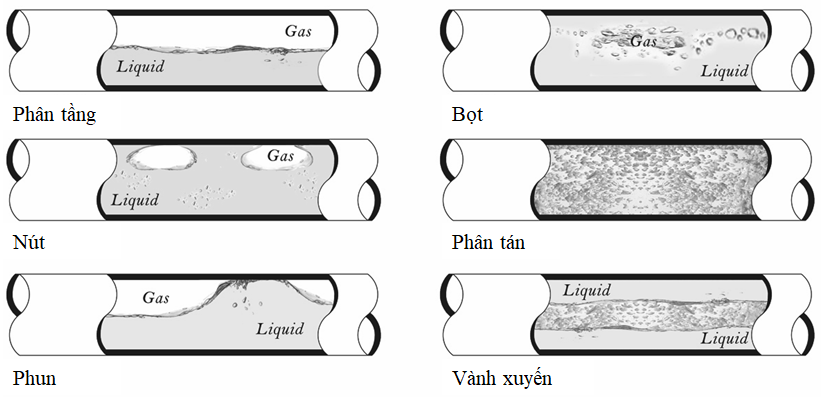
\includegraphics[scale=0.65]{Fig/horizontal_flow_regime.png}
		\caption{Chế độ dòng chảy trong ống ngang}
		\label{fig:horizontal_flow_regime}
	\end{figure}
Đối với dòng chảy đứng trong giếng, chế độ dòng chảy được thể hiện như Hình \ref{fig:vertical_flow_regime}. Chế độ dòng chảy không có dòng phân tầng mà thay vào đó là dòng chảy khuấy, dạng trung gian giữa dòng chảy nút và phân tầng. Hơn nữa, dòng chảy nút cũng có nhiều sự khác biệt so với chế độ dòng chảy trong ống ngang, thể hiện nút hình viên đạn và duy trì gần tâm dòng chảy.

Để mô tả dòng chảy thực trong đường ống hay giếng, cần phải xác định độ độ nghiêng ống để tính toán ảnh hướng đến dòng đa pha. Trong giếng đứng, do sự thay đổi áp suất liên tục từ đáy giếng đến đầu giếng, vì vậy, tất cả các chế độ dòng chảy (Hình \ref{fig:vertical_flow_regime} \cite{jansen2004modelling}) đều có thể xuất hiện.\\
	\begin{figure}[h]
		\centering
		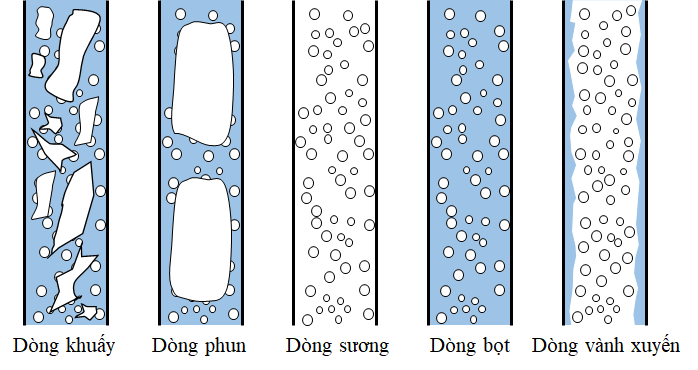
\includegraphics[scale=0.75]{Fig/vertical_flow_regime.png}
		\caption{Chế độ dòng chảy trong ống đứng}
		\label{fig:vertical_flow_regime}
	\end{figure}
Việc giải các phương trình dựa trên các định luật vật lý xây dựng bởi chế độ dòng chảy thường rất khó khăn. Trong thực tế thường sử dụng các phần mềm mô phỏng để xây dựng mô hình dòng chảy và hiệu chỉnh các thông số dòng chảy. Mỗi mô hình sẽ phù hợp với một số loại giếng nhất định.

\section{Mô hình tương quan của dòng chảy}
\subsection{Dự đoán gradient áp suất trên đường ống}

Trong hệ thống khai thác, 80\% lượng áp suất mất mát tại cột ống khai thác. Có thể nói sự thay đổi áp suất trên đường ống phụ thuộc vào 3 thành phần gồm trọng trường, sự ma sát giữa dòng lưu chất và thành ống và sự thay đổi vận tốc dòng lưu chất. Việc xác định sự thay đổi áp suất trong đường ống được thể hiện qua phương trình:
	\begin{equation}
		\left(\dfrac{dP}{dL}\right)_{total} = \left(\dfrac{dP}{dL}\right)_{el} + \left(\dfrac{dP}{dL}\right)_{f} + \left(\dfrac{dP}{dL}\right)_{acc}
	\end{equation}
	\begin{figure}[h]
		\centering
		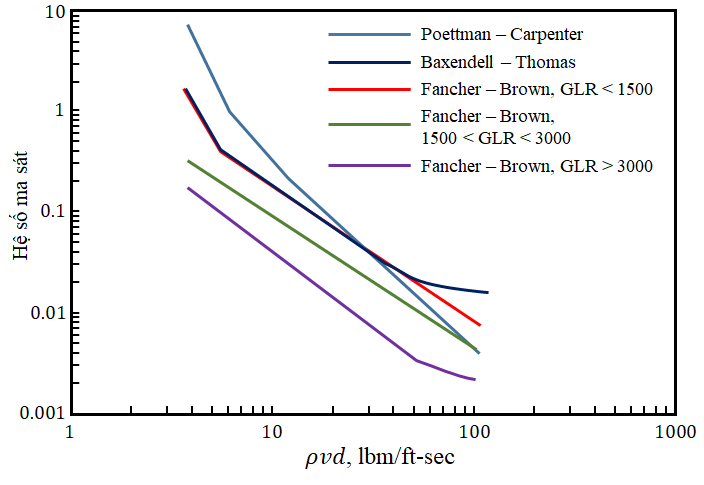
\includegraphics[scale=0.75]{Fig/category_a_friction_factor_corr.png}
		\caption[Các tương quan thực nghiệm loại “\textbf{a}”]{Các tương quan thực nghiệm loại “\textbf{a}” \cite{brill1999multiphase}}
		\label{fig:category_a_friction_factor_corr}
	\end{figure}
\newline
Để xác định gradient áp suất trên đường ống người ta đưa ra một số các mô hình thực nghiệm. Đồng thời, người ta cũng phân các tương quan thực nghiệm trên ra làm 3 loại gồm:
	\begin{itemize}
		\item Loại “\textbf{a}”: bỏ qua sự ảnh hưởng của cả sự trượt khí (slip) và chế độ dòng chảy (flow pattern) (Hình \ref{fig:category_a_friction_factor_corr})
		\item Loại “\textbf{b}”: có tính đến sự ảnh hưởng của sự trượt khí (slip), bỏ qua chế độ dòng chảy (flow pattern)
		\item Loại “\textbf{c}”: có tính đến ảnh hưởng của cả sự trượt khí (slip) và chế độ dòng chảy (flow pattern).
	\end{itemize}
Một số tương quan loại “\textbf{a}” bao gồm: \textbf{Poettmann - Carpenter, Baxendell - Thomas, Fancher - Brown}. Những phương pháp này áp dụng cho dòng chảy thẳng đứng và hỗn hợp lưu chất đồng nhất không có sự trượt khí. Xác định độ giảm áp dựa vào công thức:
	\begin{equation}
		\dfrac{dP}{dZ} = \dfrac{f\rho_{n}v_{m}^2}{2d} + \rho_{n}g
	\end{equation}
Các tương quan thực nghiệm loại “\textbf{b}” có thể kể đến như: Hagedorn và Brown, Gray, Asheim.\\

\subsection{Tương quan Hagedorn - Brown}

Tương quan \textbf{Hagedorn - Brown} được áp dụng cho giếng thẳng đứng, có chất lưu dạng hai pha. Phương trình tương quan:
	\begin{equation}
		\dfrac{dP}{dZ} = \dfrac{f\rho_{n}^2v_{m}^2}{2\rho_d} + \rho_{s}g + \dfrac{\rho_{s}\Delta v_{m}^2}{2dZ}
	\end{equation}
Để xác định sự thay đổi áp suất trên đường ống dựa vào tương quan Hagedorn và Brown, chúng ta có các bước sau:
	\begin{itemize}
		\item Bước 1: Xác định liquid holdup, $H_L$ 
		\item Bước 2: Xác định hệ số ma sát, $f$
		\item Bước 3: Xác định độ thay đổi áp suất theo chiều dài của đường ống.
	\end{itemize}

\textit{a. Xác định liquid holdup, $H_L$}

Để xác định giá trị các thành phần trong công thức người ta phải tìm cách xác định tỷ lệ lỏng (Liquid holdup, $H_L$). Trong phương pháp này, người ta không xác định tỷ lệ lỏng (Liquid holdup, $H_L$) thông qua việc đo mà thông qua tính toán. Phương pháp tính được thực hiện như sau:

\hspace*{1cm}+ Hệ số vận tốc phần lỏng:
	\begin{equation}
	N_{Lv} = v_{SL} \sqrt[4]{\dfrac{\rho_L}{g\sigma_L}}
	\end{equation}	
\hspace*{1cm}+ Hệ số vận tốc phần khí:
	\begin{equation}
	N_{gv} = v_{Sg} \sqrt[4]{\dfrac{\rho_L}{g\sigma_L}}
	\end{equation}	
\hspace*{1cm}+ Hệ số đường kính ống:
	\begin{equation}
	N_{d} = d \sqrt{\dfrac{\rho_Lg}{\sigma_L}}
	\end{equation}
\hspace*{1cm}+ Hệ số độ nhớt phần lỏng:
	\begin{equation}
	N_{L} = \mu_L \sqrt[4]{\dfrac{g}{\rho_L\sigma_L^3}}
	\end{equation}
Các đồ thị sau được sử dụng để xác định $H_L$.
	\begin{figure}[h]
		\centering
		\subfloat[\label{fig:hagedorn_brown_correlation_psi}]
			{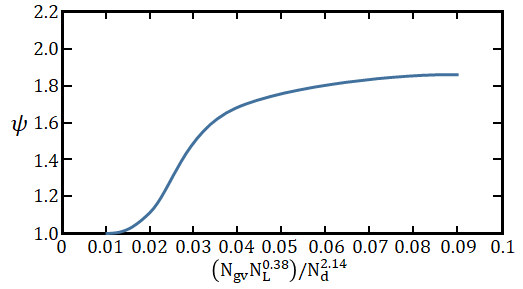
\includegraphics[scale=0.55]{Fig/hagedorn_brown_correlation_psi.png}}\hfill
		\subfloat[\label{fig:hagedorn_brown_correlation_N_Lc_N_l}]
			{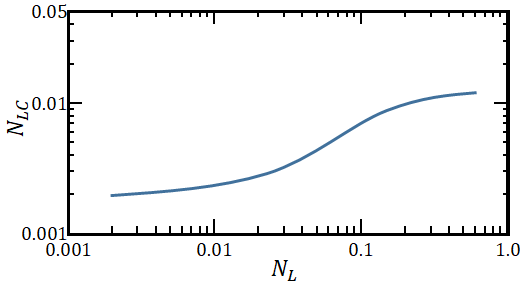
\includegraphics[scale=0.55]{Fig/hagedorn_brown_correlation_N_Lc_N_l.png}}\hfill
		\subfloat[\label{fig:hagedorn_brown_correlation_H_L_bsi}]
			{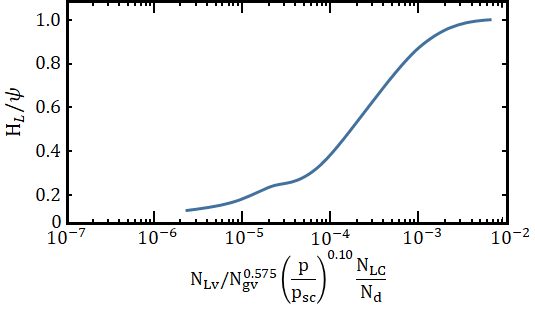
\includegraphics[scale=0.65]{Fig/hagedorn_brown_correlation_H_L_bsi.png}}
		\caption[Tỷ lệ lỏng $H_L$ trong tương quan Hagedorn - Brown]{Tỷ lệ lỏng $H_L$ trong tương quan Hagedorn - Brown \cite{brill1999multiphase}}
	\end{figure}
\newpage
\textit{b. Xác định hệ số ma sát, f}

Trong phương pháp này, người ta xác định hệ số ma sát dựa vào giản đồ Moody (Hình \ref{fig:Moody_diagram}) với số Reynolds được tính theo công thức:
	\begin{equation}
	N_{Re} = \dfrac{\rho_{n}v_{m}d}{\mu_s}
	\end{equation}
Các tương quan thực nghiệm loại “\textbf{c}” có thể kế đến như Duns - Ros, Orkiszewski, Aziz, Beggs và Brill, Mukherijee và Brill...
	\begin{figure}[h]
		\centering
		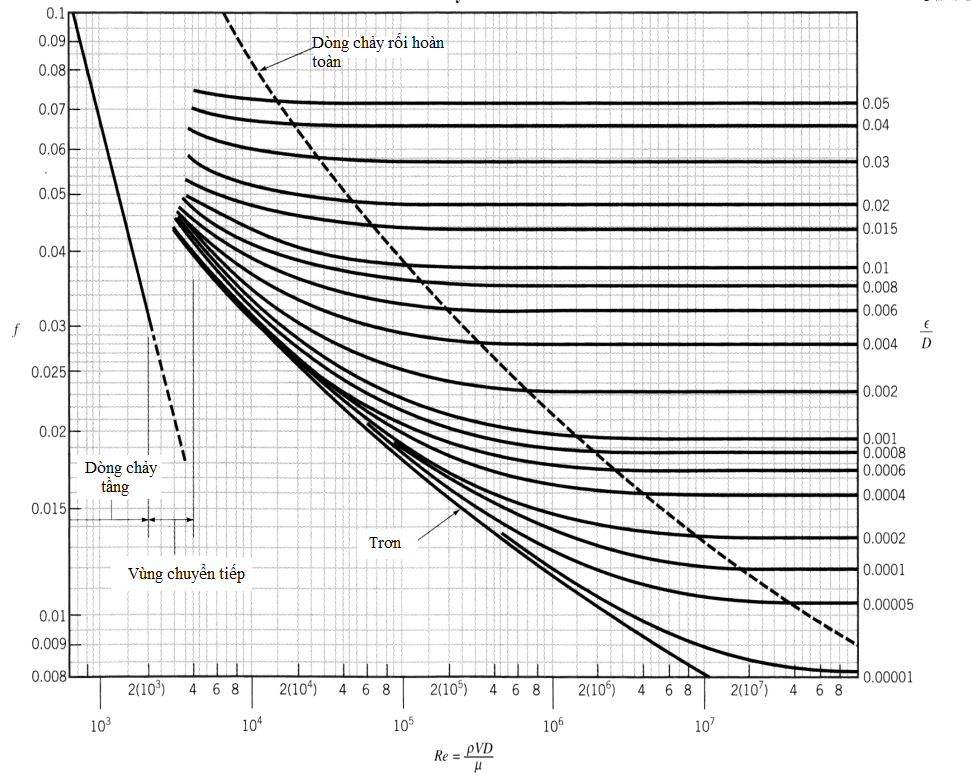
\includegraphics[scale=0.6]{Fig/Moody_diagram.png}
		\caption[Giản đồ Moody]{Giản đồ Moody \cite{brill1999multiphase}}
		\label{fig:Moody_diagram}
	\end{figure}

\subsection{Tương quan Duns - Ros}

Việc xác định chế độ dòng chảy trong đường ống bởi phương pháp được dựa trên giản đồ chế độ dòng chảy Duns và Ros. Giản đồ được chia thành 4 vùng riêng biệt, từ vùng I tới vùng III và một vùng chuyển tiếp.

Hình \ref{fig:Duns_and_Ros_flow_pattern} thể hiện chế độ dòng chảy theo Duns và Ros.
	\begin{figure}[h]
		\centering
		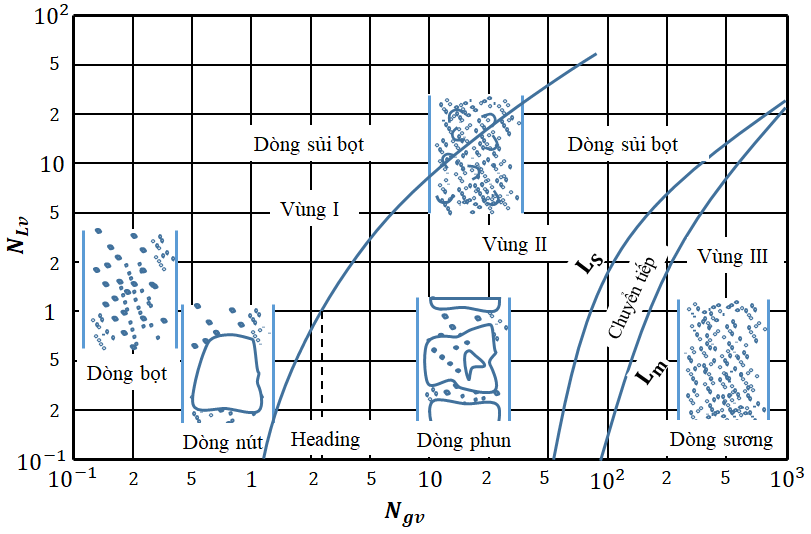
\includegraphics[scale=0.7]{Fig/Duns_and_Ros_flow_pattern.png}
		\caption[Chế độ dòng chảy theo Duns - Ros]{Chế độ dòng chảy theo Duns - Ros \cite{brill1999multiphase}}
		\label{fig:Duns_and_Ros_flow_pattern}
	\end{figure}
Cách tính toán các thông số  $N_{Lv}$ , $N_{gv}$, $N_{d}$ , $N_{L}$  đã nêu trong phương pháp của Hagedorn và Brown.

Các thông số đặc trưng cho biên của các vùng chế độ dòng chảy:

\textit{a. Giữa vùng bọt và nút (bubble/slug)}
	\begin{equation}
	N_{gv_{B/S}} = L_1 + L_2N_{Lv}
	\end{equation}
Trong đó $L_1$ và $L_2$ phụ thuộc vào $N_d$ và được thể hiện qua Hình \ref{fig:L_one_L_two_params}.
	\begin{figure}[h]
		\centering
		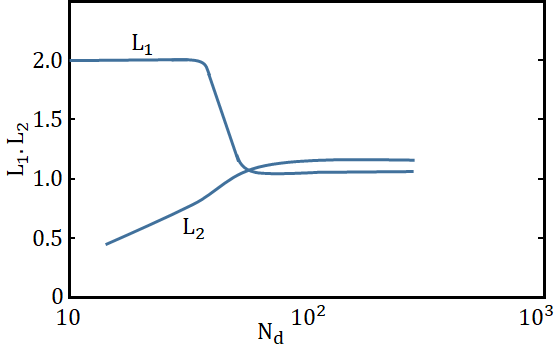
\includegraphics[scale=0.8]{Fig/L_one_L_two_params.png}
		\caption[Thông số trong chế độ dòng chảy chuyển tiếp]{Thông số trong chế độ dòng chảy chuyển tiếp \cite{brill1999multiphase}}
		\label{fig:L_one_L_two_params}
	\end{figure}
\newpage
\textit{b. Giữa vùng nút và chuyển tiếp (slug/transition)}
	\begin{equation}
	N_{gv_{S/Tr}} = 50 + 36N_{Lv}
	\end{equation}
\textit{c. Giữa vùng chuyển tiếp và phân tán (transition/mist)}
	\begin{equation}
	N_{gv_{Tr/M}} = 75 + 84N_{Lv}^{0,75}
	\end{equation}
Các bước để tính gradient áp suất trên đường ống bằng phương pháp Duns - Ros như sau:

Bước 1: Xác định hệ số đặc trưng cho vận tốc trượt, S. Hệ số này phụ thuộc vào đặc tính dòng chảy và được giải thích sau.

Bước 2: Xác định vận tốc trượt khí (slip velocity) bằng cách giải phương trình sau:
	\begin{equation}
	S = v_s\sqrt[4]{\dfrac{\rho_L}{g\sigma_L}}
	\end{equation}
Bước 3: Xác định tỷ lệ lỏng (liquid holdup) dựa vào phương trình sau:
	\begin{equation}
    v_s = v_g - v_L = \dfrac{v_{Sg}}{1-H_L}-\dfrac{v_{SL}}{H_L}
	\end{equation}
Bước 4: Xác định tỷ trọng trượt khí (slip density)
	\begin{equation}
    \rho_s = \rho_LH_L + \rho_g(1-H_L)
	\end{equation}
Bước 5: Xác định thành phần mất áp do trọng trường, $\rho_Sg$

Đối với từng chế độ dòng chảy khác nhau, sự mất mát áp suất do ma sát và sự thay đổi của vận tốc sẽ khác nhau. Cụ thể được trình bày như sau:

\textbf{Dòng chảy dạng bọt (bubble flow)}
	\begin{equation}
    S = F_1 +F_2N_Lv + F_3'\dfrac{N_{gv}}{1+N_{Lv}}
	\end{equation}
	
Trong đó: 
	\begin{equation}
   F_3' = F_3 - \dfrac{F_4}{N_d}
	\end{equation}
	
Các $F_1, F_2, F_3$ được xác định qua các đồ thị ở Hình \ref{fig:v_gas_slip_duns_ros_bubble_flow}.
	\begin{figure}[h]
		\centering
		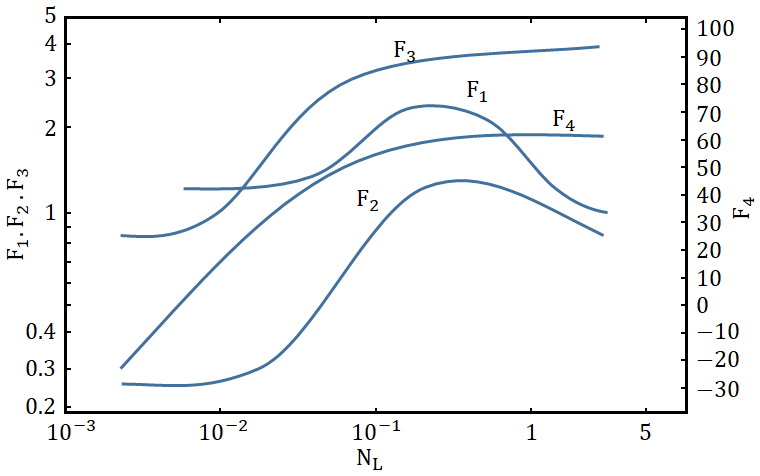
\includegraphics[scale=0.75]{Fig/v_gas_slip_duns_ros_bubble_flow.png}
		\caption[Thông số vận tốc trượt khí cho dòng chảy dạng bọt]{Thông số vận tốc trượt khí cho dòng chảy dạng bọt \cite{brill1999multiphase}}
		\label{fig:v_gas_slip_duns_ros_bubble_flow}
	\end{figure}
Thành phần mất áp bởi ma sát cho dòng chảy dạng bọt được xác định qua công thức:
	\begin{equation}
    	(\dfrac{dP}{dZ})_f = \dfrac{f\rho_Lv_{SL}v_m}{2d}
	\end{equation}
Với 
	\begin{equation}
    	f = f_1\dfrac{f_2}{f_3}
	\end{equation}
$f_1$ được xác định bằng giản đồ Moody, số Reynolds:
	\begin{equation}
    	N_{Re_L} = \dfrac{\rho_Lv_{SL}d}{\mu_L}
	\end{equation}
$f_2$ được xác định thông qua đồ thị ở Hình \ref{fig:params_for_friction_bubble_flow_duns_ros} \cite{brill1999multiphase}.
	\begin{figure}[h]
		\centering
		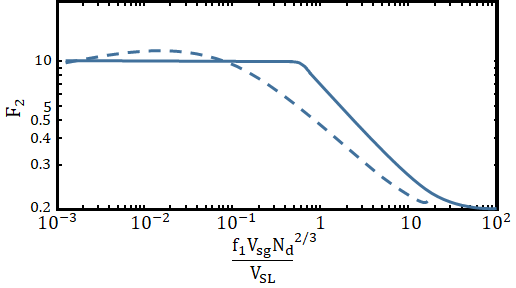
\includegraphics[scale=0.9]{Fig/params_for_friction_bubble_flow_duns_ros.png}
		\caption{Thông số cho hệ số ma sát với dòng chảy dạng bọt}
		\label{fig:params_for_friction_bubble_flow_duns_ros}
	\end{figure}
\newline
Và $f_3$ được xác định qua công thức:
	\begin{equation}
    f_3 = 1 + \dfrac{f_1}{4}\sqrt{\dfrac{v_{Sg}}{50v_{SL}}}
	\end{equation}
Đối với tương quan thực nghiệm của Duns - Ros, mất áp do sự thay đổi vận tốc được xem là không đáng kể.

\textbf{Dòng chảy dạng nút (Slug Flow)}
	\begin{equation}
    S = (1 + F_5)\dfrac{N_{gv}^{0,982}+F_6'}{(1 + F_{7}N_{Lv})^2}
	\end{equation}
Trong đó:
	\begin{equation}
F_6' = 0,029N_d + F_6
	\end{equation}

Các thông số $F_5, F_6, F_7$ được xác định thông qua đồ thị ở Hình \ref{fig:f_5_f_6_f_7_for_v_slip_gas_duns_ros} \cite{brill1999multiphase}.
	\begin{figure}[h]
		\centering
		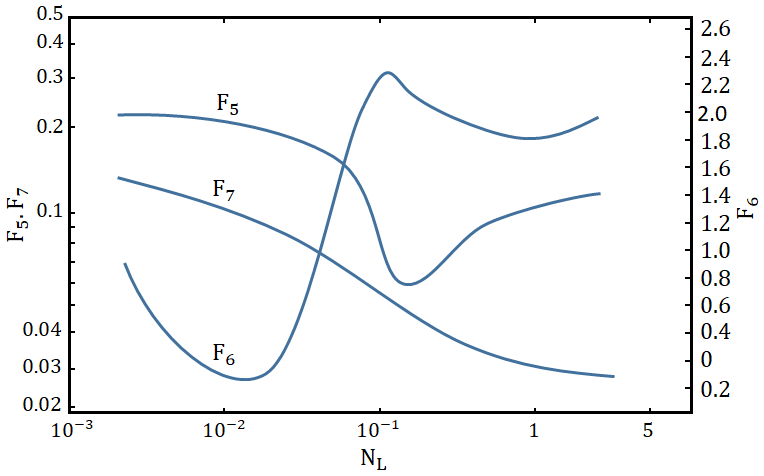
\includegraphics[scale=0.75]{Fig/f_5_f_6_f_7_for_v_slip_gas_duns_ros.png}
		\caption{Thông số tính toán cho vận tốc trượt khí của dòng chảy dạng nút}
		\label{fig:f_5_f_6_f_7_for_v_slip_gas_duns_ros}
	\end{figure}
\newline
Mất mát áp suất do thành phần ma sát được tính tương tự như cho dòng chảy dạng bọt (bubble flow). Cũng như vậy, mất mát áp suất do sự thay đổi vận tốc gần như không đáng kể cho dòng chảy dạng nút (slug flow).

\textbf{Dòng chảy dạng phân tán (Mist Flow)}

Duns và Ros cho rằng, khi lưu lương phần khí cao thì phần lỏng gần như chuyển động gần với tốc độ dòng khí. Dẫn đến hầu như không có sự trượt khí xảy ra. Vì vậy, $S=0, V_s=0 $ và $ H_L = \lambda_L$. Khối lượng riêng hỗn hợp cho việc tính mất mát áp suất do trọng trường được xác định theo công thức:
	\begin{equation}
    \rho_n=\rho_L\lambda_L+\rho_g(1-\lambda_L)
	\end{equation}
	
Mất mát áp suất do ma sát được tính theo công thức: 
	\begin{equation}
     (\dfrac{dP}{dZ})_f = \dfrac{f\rho_gv_{Sg}^2}{2d}
	\end{equation}

Trong đó hệ số ma sát được xác định bằng giản đồ Moody, với hệ số Reynold:
	\begin{equation}
     N_Re_g=\dfrac{\rho_gv_{Sg}d}{\mu_g}
    \end{equation}
    
Duns và Ros nói rằng, độ nhám của thành ống đối với dòng chảy phân tán phụ thuộc vào độ dày của lớp phủ trên bề mặt thành ống. Chính do sự không bằng phẳng trên bề mặt lớp phủ của thành ống sẽ làm tăng ứng suất cắt giữa dòng khí và lớp phủ đó và kết quả hiện tương này gây ra mất mát áp suất. Hiện tượng này còn phụ thuộc vào độ nhớt của phần lỏng trong dòng lưu chất và thể hiện qua số Weber và hệ số phụ thuộc vào độ nhớt.
 	\begin{equation}
     N_{We}= \dfrac{\rho_gv_{Sg}^2\epsilon}{\sigma_L}
    \end{equation}
    
    \begin{equation}
    N_\mu=\dfrac{\mu_L^2}{\rho_L\sigma_L\epsilon}
    \end{equation}
    
   	\begin{figure}[h]
   		\centering
   		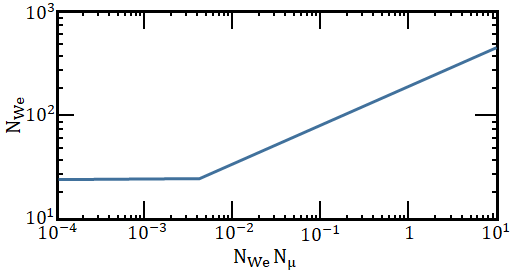
\includegraphics[scale=0.9]{Fig/params_for_envelop_wall_pipe.png}
   		\caption[Thông số đặc trưng cho lớp phủ thành ống]{Thông số đặc trưng cho lớp phủ thành ống \cite{brill1999multiphase}}
   		\label{fig:params_for_envelop_wall_pipe}
   	\end{figure}

\hspace*{1cm}+ Khi $N_{We}N_\mu\leq0,005$ thì $\dfrac{\epsilon}{d}= \dfrac{0,0749\sigma_L}{\rho_gv_{Sg}^2d}$\\

\hspace*{1cm}+ Khi $N_{We}N_\mu>0,005$ thì $\dfrac{\epsilon}{d}= \dfrac{0,3713\sigma_L}{\rho_gv_{Sg}^2d}(N_{We}N_\mu)^{0,302}$

Hệ số ma sát $f$ được xác định qua công thức:
   	\begin{equation}
    	f = 4\left\{\dfrac{1}{\left[4log_{10}\left(0.27\dfrac{\epsilon}{d}\right)\right]}+0.067\left(\dfrac{\epsilon}{d}\right)^{1.73}\right\}
    \end{equation}
   
Khi độ dốc của lớp phủ trên bề mặt thành ống tăng thì mắt cắt ngang của đường ống sẽ bị giảm. Khi đó theo Duns và Ros, sự mất áp do ma sát sẽ được tính theo $d-\epsilon$ thay vì tính theo d và $v_{Sg}$ được thay bằng $v_{Sg}d^2/(d-\epsilon)^2$ trong tấc cả các phép tính.

Mất áp do sự thay đổi vận tốc cho dòng chảy phân tán được xác định qua công thức:
   \begin{equation}
   \left(\dfrac{dP}{dZ}\right)_{acc}= \dfrac{v_mv_{Sg}\rho_n}{p} \left(\dfrac{dP}{dZ}\right)
    \end{equation}

\textbf{Vùng chuyển tiếp (Transition)}

Công thức tính mát mát áp suất với dòng chảy có dạng thuộc vùng chuyển tiếp được tính theo công thức:
   	\begin{equation}
   		\left(\dfrac{dP}{dZ}\right)_{t}= A\left(\dfrac{dP}{dZ}\right)_{slug}+(1-A)\left(\dfrac{dP}{dZ}\right)_{mist}
	\end{equation}
    
    
Với: $A = \dfrac{N_{gv_{Tr/M}}-N_{gv}}{N_{gv_{Tr/M}}-N_{gv_{S/Tr}}}$

Để tăng độ chính xác cho tính toán người ta thay khối lượng của phần khí bằng khối lượng riêng biểu kiến: $\rho_g'=\dfrac{\rho_gN_{gv}}{N_{gv_{Tr/M}}}$\\

\subsection{Tương quan Beggs và Brill}

Công thức xác định gradient áp suất được Beggs và Brill đề xuất:
	\begin{equation}
   		\dfrac{dP}{dZ}= \dfrac{\dfrac{f\rho_nv_m^2}{2d}+\rho_sgsin\theta}{1-E_k}
    \end{equation}

Với $E_k=\dfrac{v_mv_{Sg}\rho_n}{p}$, $\rho_s=\rho_LH_{L(\theta)}+\rho_g(1-H_{L(\theta)})$

\textit{Chế độ dòng chảy}

Các phương trình biên của các kiểu dòng chảy chuyển tiếp được hiệu chỉnh như sau:

$L_1=316\lambda_L^{0,302}$\\
$L_2=0,000925\lambda_L^{-2,468}$\\
$L_3=0,10\lambda_L^{-1,452}$\\
$L_4=0,5\lambda_L^{-6,738}$

Các chế độ dòng chảy trong ống nằm ngang được được thể hiện trong Hình \ref{fig:horizontal_flow_regime}.
	\begin{figure}[h]
		\centering
		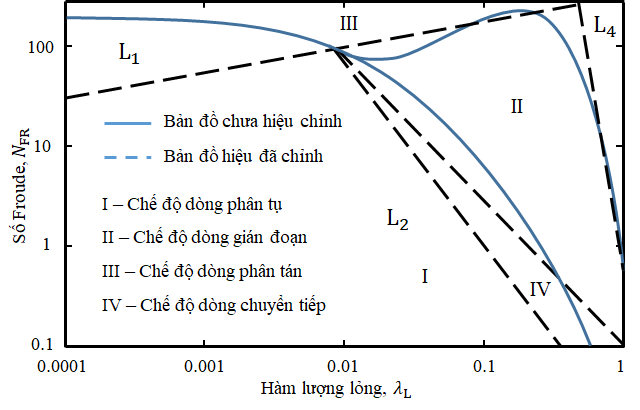
\includegraphics[scale=0.75]{Fig/liquid_holdup_gamma_l.png}
		\caption[Bản đồ phân vùng chế độ dòng chảy]{Bản đồ phân vùng chế độ dòng chảy \cite{brill1999multiphase}}
		\label{fig:liquid_holdup_gamma_l}
	\end{figure}
\newline
Những bất đẳng thức sau sử dụng để xác định kiểu dòng chảy tồn tại trong ống ngang:
	\begin{itemize}
		\item Dòng chảy tách rời (Segregated):\\
		$\lambda_L<0,01$ và $N_{Fr}<L_1$ hoặc $\lambda_L\ge0,01$ và $N_{Fr}<L_2$
		\item Dòng chảy chuyển tiếp (Transition):\\
		$\lambda_L\ge0,01$ và $L_2\leq N_{Fr}\leq L_3$
		\item Dòng chảy gián đoạn (Intermittern):\\
		$0,01\leq\lambda_L<0,4$ và $L_3<N_{Fr}\leq L_1 $
		\item Dòng chảy phân tán (Distributed):\\
		$\lambda_L<0,4$ và $N_{Fr}\ge L_1$ hoặc $\lambda_L\ge 0,4$ và $N_{Fr}>L_4$
	\end{itemize}

\textbf{Xác định tỷ lệ lỏng ($H_L$)}

Giá trị tỷ lệ lỏng được tính theo trường hợp ống nằm ngang, sau đó sẽ được hiệu chỉnh theo góc nghiêng thực tế của ống.
	\begin{figure}[h]
		\centering
		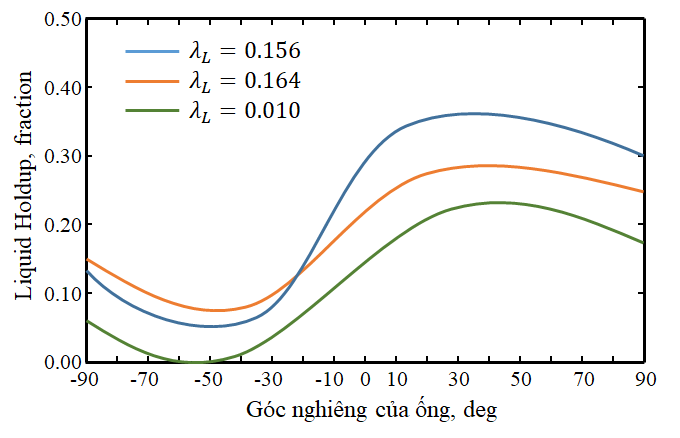
\includegraphics[scale=0.75]{Fig/h_l_vs_inclination_pipe.png}
		\caption{Quan hệ giữa hàm hượng lỏng với góc nghiêng của ống}
		\label{fig:h_l_vs_inclination_pipe}
	\end{figure}
\newline
Hình \ref{fig:h_l_vs_inclination_pipe} \cite{brill1999multiphase} là đồ thị thể hiện mối tương quan giữa $H_L$ và độ nghiêng ống. Người ta nhận rằng $H_L$ đạt giá trị lớn nhất ở độ nghiêng $+50^{\circ}$ so với phương ngang và nhỏ nhất ở $-50^{\circ}$.

Tỷ lệ lỏng theo phương ngang được tính theo công thức:\\
+) Với $H_{L(0)}\ge\lambda_L$
	\begin{equation}
   		H_{L(0)}=\dfrac{a\lambda_L^b}{N_{Fr}^c}
    \end{equation}
Với các thông số a, b, c được tra tại Bảng \ref{tab:dependent_params_1}.
\begin{table}[h]
\caption[Tham số phụ thuộc ($H_{L(0)} \ge \lambda_L$)]{Tham số phụ thuộc ($H_{L(0)} \ge \lambda_L$) \cite{brill1999multiphase}}\label{tab:dependent_params_1}
\begin{tabularx}{\textwidth}{@{}XXXX@{}}
\toprule
Chế độ dòng chảy & a     & b      & c       \\ \midrule
Dòng tách rời    & 0.980 & 0.4846 & 0.0868  \\
Dòng gián đoạn   & 0.845 & 0.5351 & 0.0173  \\
Dòng phân tán    & 1.065 & 0.5824 & 0.00609 \\ \bottomrule
\end{tabularx}
\end{table}

+) Với $H_{L(0)} \ge \lambda_L$\\
Tỷ lệ lỏng có xét đến góc nghiêng được xác định:
	\begin{equation}
   		H_{L(\theta)}= H_{L(0)}\psi
    \end{equation}
   
Trong đó: $\psi= 1,0 + C[sin(1,8\theta)-0,333sin^3(1,8\theta)]$\\
Khi $\theta$  là góc thực của ống so với phương ngang thi C được xác định:\\
$C=(1-\lambda_L)ln(e\lambda_L^fN_{Lv}^gN_{Fr}^h)$\\
Với điều kiện $C \ge 0$. Các hệ số e, f, g, h được xác định theo Bảng \ref{fig:dependent_params_2}.

Đối với kiểu dòng chảy trong vùng chuyển tiếp (Transition). Thì $H_L$ được nội suy giữa vùng dòng tách rời và dòng chảy gián đoạn.
	\begin{equation}
   		H_{L(\theta)_{Tr}}=AH_{L(\theta)_{Seg}} + (1-A)H_{L(\theta)_{Int}}
    \end{equation}
    
Trong đó: $A= \dfrac{L_3-N_{Fr}}{L_3-L_2}$

Hệ số ma sát được xác định bởi công thức:
	\begin{equation}
		f / f_n = e^s
	\end{equation}
	\begin{equation}
		s=\dfrac{ln(y)}{-0,0523+3,182lny-0,8725(lny)^2+0,01853(lny)^4}
	\end{equation}
	\begin{equation}
		y=\dfrac{\lambda_L}{H_{L(\theta)}^2}
	\end{equation}
Nếu $1<y<1,2$
	\begin{equation}
		s=ln(2,2y-1,2)
	\end{equation}

Với $f_n$ được xác định từ giản đồ Moody, hoặc từ công thức:

+) Đối với chế độ dòng chảy tầng $(N_{Re}<2300)$
	\begin{equation}
		f_n=\dfrac{64\mu}{N_{Re}}
	\end{equation}
+) Đối với dòng chảy chuyển tiếp $(2300<N_{Re}<3000)$
	\begin{equation}
		f_n=(0,16N_{Re}-13).10^{-4}
	\end{equation}
+) Đối với chế độ chảy rối $(3000<N_{Re}<3.10^6)$
	\begin{equation}
		f_n=0,0056 + 0,5N_{Re}^{-0,32}
	\end{equation}
Trong đó:
	\begin{equation}
		N_{Re}=\dfrac{\rho_{ns}v_md}{\mu_m}
	\end{equation}

\begin{table}[h]
\caption[Tham số phụ thuộc ($H_{L(0)} < \lambda_L$))]{Tham số phụ thuộc ($H_{L(0)} < \lambda_L$)) \cite{brill1999multiphase}}\label{fig:dependent_params_2}
\begin{tabularx}{\textwidth}{@{}XXXXX@{}}
\toprule
Chế độ dòng chảy                                                               & e         & f           & g           & h          \\ \midrule
Dòng tách rời\\ (Uphill)   & 0.0l1     & -3.6780     & 3.539       & -1.613     \\
Dòng gián đoạn\\ (Uphill) & 2.96      & 0.305       & -0.4473     & 0.0978     \\
Dòng phân tán\\ (Uphill)   & \multicolumn{4}{c}{C = 0, $\psi$ = 1} \\
Tất cả (Downhill)                                                              & 4.7       & -0.3692     & 0.1244      & -0.5056    \\ \bottomrule
\end{tabularx}
\end{table}

\chapter{TỐI ƯU HÓA KHAI THÁC CHO GIẾNG DẦU}
\section{Lưu lượng khai thác}

Hệ thống dòng chảy giữa vỉa và đầu tubing có thể được chia thành:
	\begin{itemize}
		\item Dòng chảy từ vỉa vào giếng
		\item Dòng chảy từ đáy giếng lên đầu tubing
	\end{itemize}
Dòng chảy từ vỉa bị tác động bởi:
	\begin{itemize}
		\item Áp suất vỉa
		\item Tính chất vỉa
		\item Hệ số nhiễm bẩn - bao gồm cả nhiễm bẩn do hoàn thiện giếng
		\item Đặc tính của lưu chất vỉa.
	\end{itemize}
Tuy nhiên như chúng ta đã biết tất cả những ảnh hưởng có thể đưa về một mối quan hệ đơn – đường dòng vào của giếng. Giả sử chúng ta có đường dòng vào tuyến tính với chỉ số khai thác J thì:
	\begin{equation}
		p_{wf} = p_R + \dfrac{q_{o,sc}}{J}
	\end{equation}
Với $q_{o,sc}$ mang giá trị dương cho giếng bơm ép và âm cho giếng khai thác. Tương tự dòng chảy từ đáy giếng lên đầu tubing bị tác động bởi:
	\begin{itemize}
		\item Kích thước tubing và các thông số hoàn thiện giếng
		\item Chế độ dòng chảy trong giếng
		\item Tính chất lưu chất.
	\end{itemize}
Những tác động này không thể đưa về một quan hệ đơn mà dự đoán áp suất thất thoát trong tubing. Tuy nhiên nếu chúng ta đã biết áp suất đầu tubing (THP) \nomenclature{THP}{Áp suất đầu tubing} và các yếu tố như đường kính tubing thì có thể xây dựng đường cong áp suất đầu vào như một hàm phụ thuộc vào lưu lượng dòng chảy.
	\begin{equation}
		p_{wf} = F_{ip}(q_{o,sc})
	\end{equation}
Với $F_{ip}$ là hàm thể hiện đường cong áp suất đầu vào. Ngoài ra hàm $F_{ip}$ còn phụ thuộc vào các thông số như THP, đường kính tubing, GLR \nomenclature{GLR}{Tỉ lệ khí lỏng} và hàm lượng nước trong sản phẩm khai thác.
	\begin{figure}[h]
		\centering
		\subfloat[Đường đặc tính dòng vào với PI là hằng số\label{fig:ipr_vs_const_pi}]
			{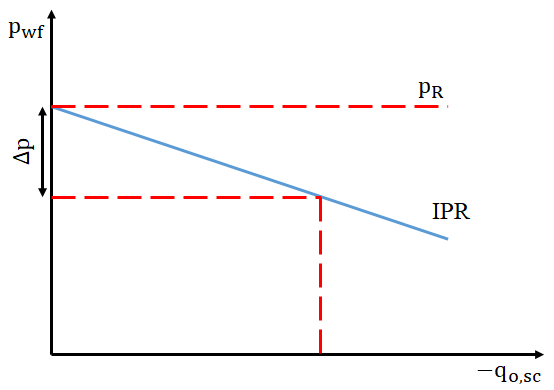
\includegraphics[scale=0.55]{Fig/ipr_vs_const_pi.png}}\hfill
		\subfloat[Áp suất đầu vào với lưu lượng khai thác thay đổi\label{fig:intake_pressure_vs_pi}]
			{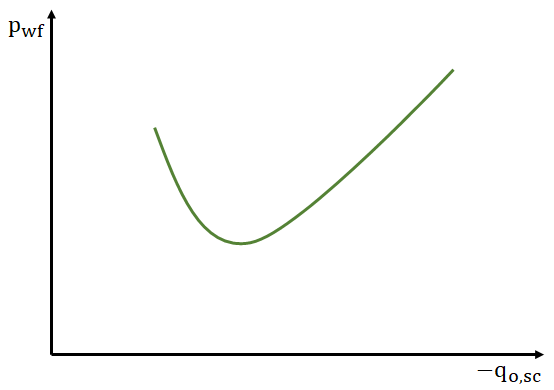
\includegraphics[scale=0.55]{Fig/intake_pressure_vs_pi.png}}\hfill
		\caption[Các đường đặc tính vận hành]{Các đường đặc tính vận hành \cite{jansen2004modelling}}
	\end{figure}
\newline
Đường dòng vào được thể hiện trong Hình \ref{fig:ipr_vs_const_pi}, đường cong áp suất đầu vào được thể hiện trong Hình \ref{fig:intake_pressure_vs_pi}. Thực tế, đường đặc tính vận hành chính là sự kết hợp giữa hai đường cong đã nêu đồng thời là cơ sở để xây dựng phương pháp phân tích điểm nút (Hình \ref{fig:mix_between_intake_and_ipr} \cite{jansen2004modelling}). Hai đường cong có hai điểm giao nhau, điểm giao nhau bên phải là
điểm vận hành ổn định và cho chúng ta lưu lượng dòng chảy thực $q_{o,sc}$ và áp suất đáy giếng thực $p_{wf}$, điểm giao nhau bên trái là điểm không ổn định vì vậy là điểm vận hành không có thực.

Đường áp suất đầu vào được suy ra từ áp suất đầu giếng cố định, nếu chúng ta giảm $p_{wh}$ và $p_{wf}$ cũng giảm thì đường áp suất đầu vào sẽ trượt xuống, vì vậy đường cong này có thể thay đổi hình dạng của nó vì chế độ dòng chảy trong tubing có thể thay đổi. Nếu như điểm vận hành ổn định dịch chuyển sang phải sẽ làm tăng lưu lượng dòng chảy. Ngược lại, nếu chúng ta tăng áp suất đầu giếng thì lưu lượng dòng chảy sẽ giảm và nếu chúng ta tăng áp suất đầu giếng quá lớn thì giếng sẽ không cho dòng nữa.
	\begin{figure}[h]
		\centering
		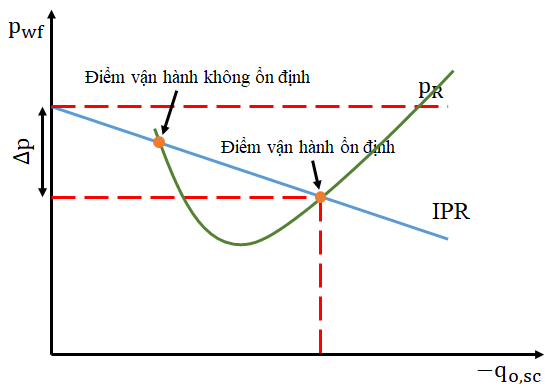
\includegraphics[scale=0.8]{Fig/mix_between_intake_and_ipr.png}
		\caption{Sự kết hợp đường dòng vào và đường áp suất dầu vào}
		\label{fig:mix_between_intake_and_ipr}
	\end{figure}
\newline
Tương tự, điểm vận hành cũng sẽ bị ảnh hưởng bởi áp suất vỉa suy giảm sau một thời gian khai thác. Trong trường hợp không thể giảm áp suất đầu giếng, có thể duy trì hoạt động khai thác bằng cách thay đổi kích thước tubing để làm giảm tổn thất áp suất trong đường ống tubing, kích thước tubing phụ thuộc vào các yếu tố như hàm lượng nước trong sản phẩm và tỉ số khí dầu. Một sự lựa chọn khác là chuyển sang hình thức khai thác cơ học như gas lidt, bơm điện ly tâm chìm ESP \nomenclature{ESP}{Bơm điện ly tâm chìm} hoặc bơm gật gù.

Ở phần trên chúng ta giả sử THP và áp suất vỉa là hằng số và tính toán lưu lượng dòng chảy từ áp suất suy giảm qua tubing và vỉa. Tuy nhiên THP thường sẽ thay đổi với lưu lượng dòng chảy, để phân tích tác động này chúng ta cũng cần xét đến đường dòng của các thiết bị bề mặt từ đầu giếng cho đến điểm có thể giả sử là áp suất duy trì tại một giá trị không đổi (thường là bình tách đầu tiên). Trong vỉa chúng ta vẫn giả sử áp suất là một hằng số hoặc là thay đổi rất chậm so với thời gian khai thác. Cuối cùng, vấn đề của chúng ta là xác định lưu lượng dòng chảy bằng việc xét áp suất suy giảm qua những thiết bị sau:
	\begin{itemize}
		\item Vỉa (bao gồm vùng cận đáy giếng và hoàn thiện giếng)
		\item Dòng chảy từ đáy giếng lên đầu tubing
		\item Dòng chảy qua van tiết lưu
		\item Dòng chảy qua đường ống và thiết bị bề mặt.
	\end{itemize}
Với các giá trị áp suất trong vỉa và đầu bình tách không đổi đồng thời thành phần chất lưu không đổi.

	\begin{figure}[h]
		\centering
		\subfloat[Áp suất đầu tubing\label{fig:too_high_thp}]
			{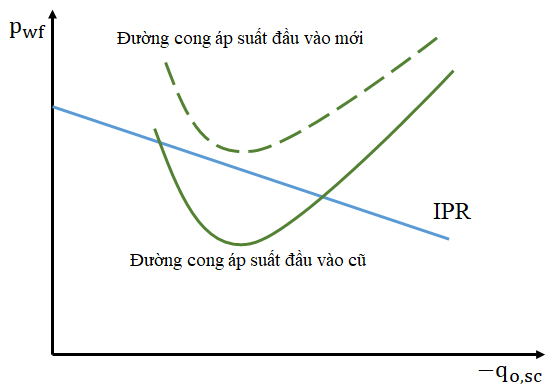
\includegraphics[scale=0.55]{Fig/too_high_thp.png}}\hfill
		\subfloat[Đặc tính van tiết lưu\label{fig:choke_performance_curve}]
			{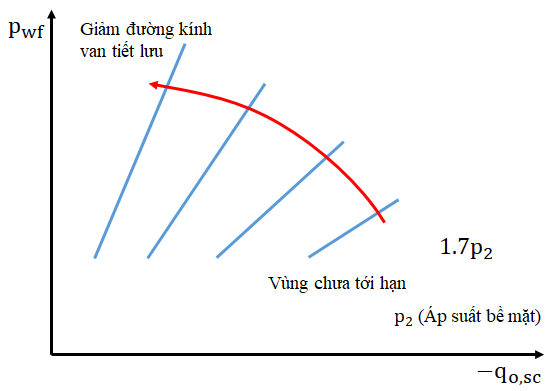
\includegraphics[scale=0.55]{Fig/choke_performance_curve.png}}\hfill
		\caption[Ảnh hưởng áp suất và đường kính van tiết lưu]{Ảnh hưởng áp suất và đường kính van tiết lưu \cite{jansen2004modelling}}
	\end{figure}

Với một đường dòng vào cho trước đồng thời lưu lượng dòng chảy và áp suất đáy giếng đã được xác định, dùng áp suất này kết hợp với đường kính tubing đã cho, GOR và hàm lượng nước trong sản phẩm thì áp suất dòng trong tubing ($p_{tf}$) có thể được xác định từ phân tích sụt áp trong giếng bằng việc sử dụng máy tính hoặc đường cong gradient. Mối quan hệ giữa lưu lượng dòng chảy $q_{o,sc}$ và $p_{tf}$ được gọi là đường đặc tính tubing. Phương pháp sử dụng đường cong gradient được thể hiện trong Hình \ref{fig:tubing_performance_vs_intake_pressure}.

Đường đặc tính tubing không chỉ dựa trên khả năng vận chuyển chất lưu của tubing mà còn chứa đặc tính của vỉa và hoàn thiện giếng thông qua dòng vào từ vỉa, nếu áp suất vỉa suy giảm thì đường đặc tính tubing sẽ thay đổi.

Dòng chảy qua van tiết lưu bị chi phối bởi đường đặc tính van tiết lưu  (Hình \ref{fig:choke_performance_curve}). Giả sử dòng chảy ở trên điểm tới hạn, đường đặc tính van tiết lưu có thể kết hợp với đường đặc tính tubing để xác định điểm vận hành tại đầu tubing. Mối tương quan giữa đường kính với đường đặc tính van tiết lưu được thể hiện trong đồ thị Hình \ref{fig:tubing_vs_choke_performance}. Giả thiết rằng áp suất sau van tiết lưu không đổi và bằng với áp suất đầu bình tách $p_m$, một lần nữa chúng ta có hai điểm vận hành, tuy nhiên trong thực tế trường hợp này ít xảy ra. Có thể khẳng định rằng điểm vận hành tại lưu lượng thấp hơn thường không ổn định.

	\begin{figure}[h]
		\centering
		\subfloat[Đặc tính tubing với áp suất đầu vào\label{fig:tubing_performance_vs_intake_pressure}]
			{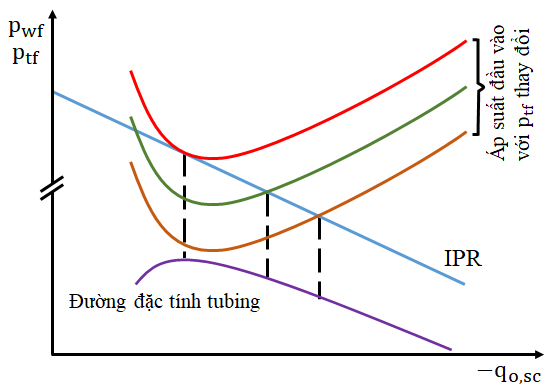
\includegraphics[scale=0.55]{Fig/tubing_performance_vs_intake_pressure.png}}\hfill
		\subfloat[Đặc tính tubing với kích thước van tiết lưu\label{fig:tubing_vs_choke_performance}]
			{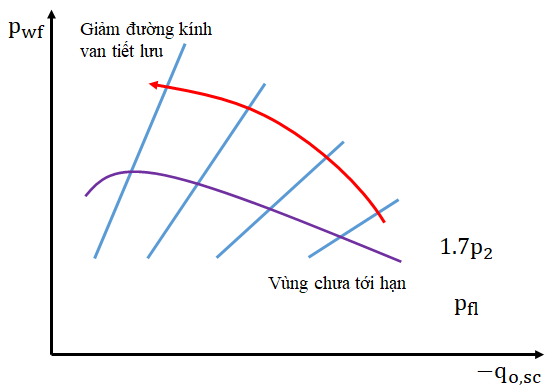
\includegraphics[scale=0.55]{Fig/tubing_vs_choke_performance.png}}\hfill
		\caption[Đường đặc tính tubing]{Đường đặc tính tubing \cite{jansen2004modelling}}
	\end{figure}

\section{Tối ưu hóa khai thác}
\subsection{Tối ưu hóa khai thác trong thời gian ngắn}

\textit{a. Cải thiện đường đặc tính dòng vào}

Nếu lưu lượng khai thác của giếng giảm quá nhiều, cần phải thực hiện xử lý cận đáy giếng để cải thiện đường dòng vào đồng thời cũng có thể thực hiện bắn mở vỉa bổ xung. Để có thể cải thiện đường dòng vào cần phải biết được những gì đang xảy ra ở đáy giếng, Hình \ref{fig:enhance_ipr_with_perforation} thể hiện đường dòng vào trước và sau khi thực hiện xử lý cận đáy giếng. Quá trình cải thiện đường đặc tính dòng vào thường kèm theo nhiều chi phí phát sinh làm tăng chi phí vận hành của giếng.

\textit{b. Thay đổi đường kính trong tubing hoặc van tiết lưu}

Tăng hoặc giảm đường kính trong tubing hay van tiết lưu có thể cải thiện lưu lượng khai thác. Chi phí thay đổi tubing thường khá cao và cần phải thực hiện hiệu chỉnh nhiều thiết bị liên quan, đồng thời chỉ thay đổi khi đảm bảo được khả năng vận hành lâu dài với tubing mới. Thay đổi van tiết lưu là phương pháp được ưu tiên sử dụng hơn, giới hạn vận hành của van tiết lưu được thể hiện trong Hình \ref{fig:min_max_choke_size}.

	\begin{figure}[h]
		\centering
		\subfloat[Cải thiện đường dòng vào\label{fig:enhance_ipr_with_perforation}]
			{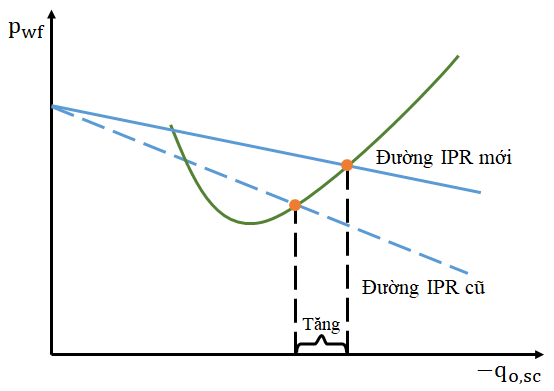
\includegraphics[scale=0.55]{Fig/enhance_ipr_with_perforation.png}}\hfill
		\subfloat[Giới hạn làm việc của van tiết lưu\label{fig:min_max_choke_size}]
			{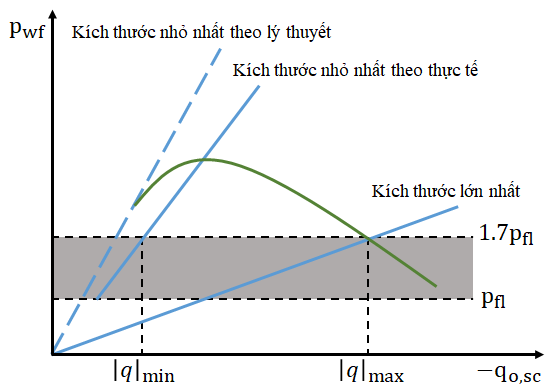
\includegraphics[scale=0.55]{Fig/min_max_choke_size.png}}
		\caption[Cải thiện lưu lượng khai thác trong thời gian ngắn]{Cải thiện lưu lượng khai thác trong thời gian ngắn \cite{jansen2004modelling}}
	\end{figure}

\subsection{Tối ưu hóa khai thác trong thời gian dài}

\textit{a. Ảnh hưởng suy giảm áp suất vỉa}

Quá trình phân tích ảnh hưởng của suy giảm áp suất vỉa được thực hiện vị trí đáy giếng và dùng đường cong áp suất đầu vào. Giả sử rằng chỉ số khai thác không đổi trong khi áp suất vỉa giảm như Hình \ref{fig:effect_of_decline_res_pressure}, đường dòng vào sẽ di chuyển thẳng đứng xuống theo trục áp suất đáy giếng. Nếu áp suất vỉa giảm quá nhiều thì việc thay đổi đường kính trong tubing cần được thực hiện ngay. Thực hiện phân tích tương tự cho tubing mới để có thể xác định được thời gian vận hành của tubing so với vòng đời của giếng và dự doán chi phi vận hành kèm theo.
\newpage
	\begin{figure}[h]
		\centering
		\subfloat[Suy giảm áp suất vỉa\label{fig:effect_of_decline_res_pressure}]
			{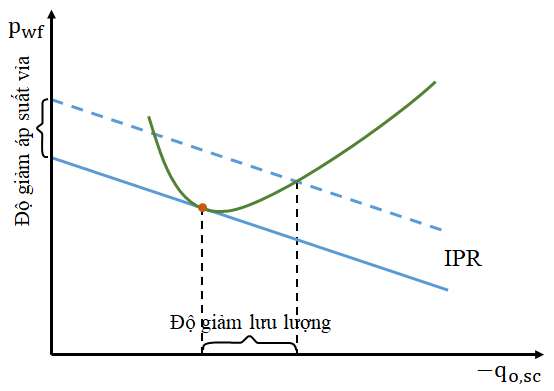
\includegraphics[scale=0.55]{Fig/effect_of_decline_res_pressure.png}}\hfill
		\subfloat[Sự thay đổi tỉ số khí dầu\label{fig:optimum_gor}]
			{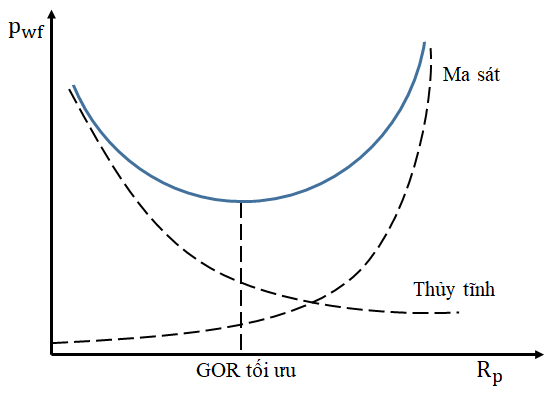
\includegraphics[scale=0.55]{Fig/optimum_gor.png}}
		\caption[Tối ưu khai thác trong thời gian dài]{Tối ưu khai thác trong thời gian dài \cite{jansen2004modelling}}
	\end{figure}

\textit{b. Lắp đặt gas lift}

Gas lift là một trong những phương pháp phổ biến nhất của hình thức khai thác cơ học, bằng cách bơm khí vào tubing, làm cột chất lỏng nhẹ hơn đồng thời tăng lưu lượng khai thác.

Trong quá trình gas lift với lưu lượng khai thác đã biết cần phải bơm khí tại giá trị tối ưu của GOR, điều này có thể hạn chế tổn thất áp suất qua tubing (Hình \ref{fig:optimum_gor}) và tăng lưu lượng khai thác lớn nhất có thể. Vì vậy, việc tìm kiếm giá trị GOR tối ưu của một giếng là cực kì quan trọng trong gas lift. Hình \ref{fig:or_of_production_well} thể hiện các giá trị GOR tối ưu thay đổi theo đường đặc tính tubing đối với lưu lượng cho trước.

Với GOR thấp, nếu THP dưới áp suất tới hạn của van tiết lưu có thể làm giếng không ổn định. Nếu thể hiện lưu lượng khai thác trên đồ thị một hàm của GOR, có thể thấy được GOR tăng dần và lưu lượng khai thác tăng đến giá trị tối đa 535 bpd với GOR 800. Trên GOR vượt qua giá trị này lưu lượng khai thác dầu bắt đầu giảm trở lại. Thêm vào đó khi thực hiện gas lift, kết quả cho thấy thời gian đầu rất hiệu quả, nhưng hiệu quả sẽ giảm dần khi nhiều khí được bơm vào tubing. 
\newpage
	\begin{figure}[h]
		\centering
		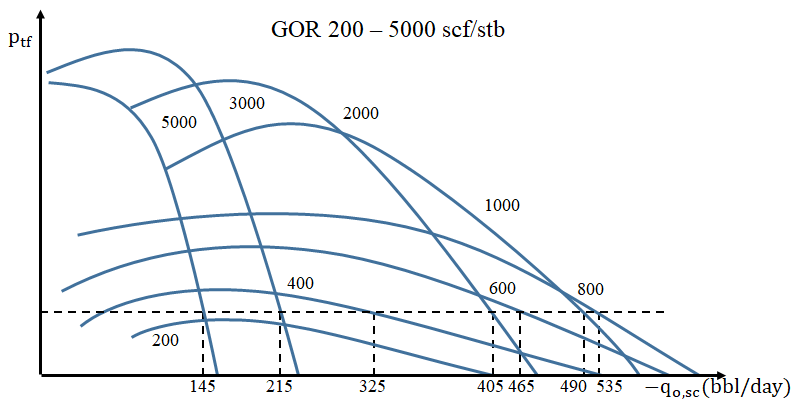
\includegraphics[scale=0.7]{Fig/gor_of_production_well.png}
		\caption[Ảnh hưởng của tỉ số khí dầu trong một giếng khai thác]{Ảnh hưởng của tỉ số khí dầu trong một giếng khai thác \cite{jansen2004modelling}}
		\label{fig:or_of_production_well}
	\end{figure}
Khi GOR tăng từ 200 đến 400 scf/stb lưu lượng khai thác tăng thêm 325 bpd, nhưng khi tăng đến 600 và 800 cho lưu lượng khai thác chỉ thêm 140 hoặc 70 bpd. Vì tính kinh tế của toàn dự án mà tỉ số khí dầu thường được giữ dưới 800 scf/stb.

\chapter{TỐI ƯU HÓA KHAI THÁC CHO GIẾNG X}

\section{Giới thiệu phần mềm PIPESIM}
PIPESIM là phần mềm mô phỏng do Schlumberger phát triển, có chức năng thiết kế và phân tích hệ thống khai thác của các giếng dầu và giếng khí. Hình \ref{fig:production_system} \cite{schlum2010pipesim} thể hiện mô hình dòng chảy đa pha từ trong vỉa qua các thành phần của hệ thống khai thác tới các thiết bị bề mặt cho phép phân tích hệ thống khai thác một cách toàn diện.
	\begin{figure}[h]
		\centering
		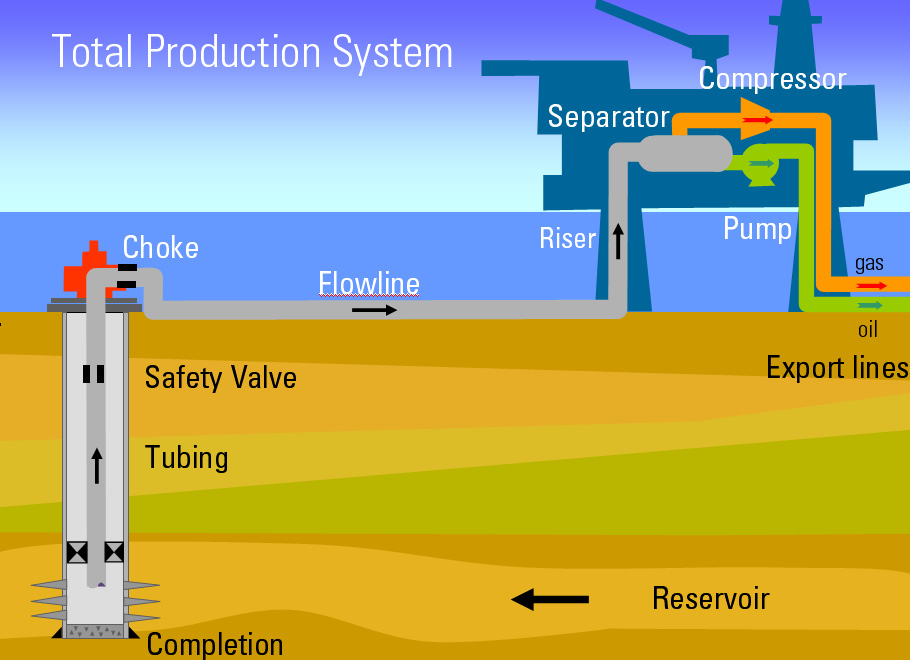
\includegraphics[scale=0.6]{Fig/production_system.png}
		\caption{Toàn bộ hệ thống cơ bản của một giếng khai thác}
		\label{fig:production_system}
	\end{figure}
\newline
PIPESIM thường được sử dụng cho phân tích vỉa, khai thác hay các thiết bị kĩ thuật. Một số chức năng chính của PIPESIM như sau:
	\begin{itemize}
		\item Phân tích các mô hình đặc tính giếng
		\item Phân tích điểm nút
		\item Thiết kế hệ thống khai thác dầu bằng khí nén
		\item Xây dựng hệ thống ống dẫn và thiết bị
		\item Phân tích đưa ra kế hoạch phát triển mỏ
		\item Tối ưu hóa khai thác.
	\end{itemize}
Phiên bản được nhóm tác giả sử dụng là PIPESIM 2017.1 có nhiều sự thay đổi về giao diện người dùng tuy nhiên các tính năng chính không có sự thay đổi nhiều so với các phiên bản cũ hơn.

\section{Mô hình khai thác của giếng X trên Pipesim}
\subsection{Dữ liệu đầu vào của giếng X}

Các thông số đầu vào của mô hình bao gồm thông số vỉa, lưu chất vỉa (Black-Oil), tubing, khoan định hướng, ống chống, các thiết bị bề mặt, các thiết bị lòng giếng, khai thác nhân tạo, hoàn thiện giếng và thông số truyền nhiệt được thể hiện qua các Bảng \ref{tab:reservoir_data} đến Bảng \ref{tab:surface_equipment}.

\begin{table}[h]
\caption{Thông số vỉa}\label{tab:reservoir_data}
\begin{tabularx}{\textwidth}{@{}XXX@{}}
\toprule
Thông số            & Dữ liệu & Đơn vị        \\ \midrule
Áp suất vỉa    & 3600 & psia        \\
Nhiệt độ vỉa & 200  & degF        \\
Chỉ số khai thác      & 9.4  & STB/(d.psi) \\ \bottomrule
\end{tabularx}
\end{table}

\begin{table}[h]
\caption{Tính chất lưu chất vỉa}\label{tab:fluid_properties}
\begin{tabularx}{\textwidth}{@{}XXX@{}}
\toprule
Thông số & Dữ liệu & Đơn vị    \\ \midrule
Watercut   & 10   & \%      \\
GOR        & 500  & SCF/STB \\
Tỉ trọng khí    & 0.8  & S.G     \\
Tỉ trọng nước  & 1.05 & S.G     \\
API        & 36   & dAPI    \\ \bottomrule
\end{tabularx}
\end{table}
\nomenclature{GOR}{Tỉ số khí dầu}

\begin{table}[h]
\caption{Các thông số của tubing}\label{tab:tubing_params}
\begin{tabularx}{\textwidth}{@{}XXX@{}}
\toprule
Thông số         & Dữ liệu & Đơn vị \\ \midrule
Độ sâu đo        & 8600    & ft     \\
Đường kính ngoài & 4.5     & in     \\
Đường kính trong & 3.476   & in     \\
Độ dày thành ống & 0.271   & in     \\
Độ nhám          & 0.001   & in     \\ \bottomrule
\end{tabularx}
\end{table}

\begin{table}[h]
\caption{Các thông số khoan định hướng}\label{tab:wellbore_data}
\begin{tabularx}{\textwidth}{@{}XX@{}}
\toprule
Độ sâu đo đạt (ft) & Độ sâu thực (ft) \\ \midrule
0       & 0        \\
1000    & 1000     \\
2500    & 2450     \\
5000    & 4850     \\
7500    & 7200     \\
9000    & 8550     \\ \bottomrule
\end{tabularx}
\end{table}

\begin{table}[h]
\caption{Các thông số truyền nhiệt}\label{tab:heat_transfer}
\begin{tabularx}{\textwidth}{@{}XX@{}}
\toprule
Độ sâu thực (ft) & Nhiệt độ môi trường (degF) \\ \midrule
0                & 50                         \\
8550             & 200                        \\ \bottomrule
\end{tabularx}
\end{table}

\begin{table}[h]
\caption{Thiết bị khai thác nhân tạo}\label{tab:gaslift_valve}
\begin{tabularx}{\textwidth}{@{}XXXX@{}}
\toprule
Tên        & Độ sâu đo (ft) & Lưu lượng bơm ép & Đơn vị  \\ \midrule
Bơm ép khí & 8000           & 0.1              & mmscf/d \\ \bottomrule
\end{tabularx}
\end{table}

\begin{table}[h]
\caption{Các thông số của ống chống}\label{tab:casing_data}
\begin{tabularx}{\textwidth}{@{}XXX@{}}
\toprule
Thông số         & Dữ liệu & Đơn vị \\ \midrule
Độ sâu đo        & 9000    & ft     \\
Đường kính ngoài & 8.625   & in     \\
Đường kính trong & 7.511   & in     \\
Độ dày thành ống & 0.557   & in     \\
Độ nhám          & 0.001   & in     \\ \bottomrule
\end{tabularx}
\end{table}

\begin{table}[h]
\caption{Các thiết bị lòng giếng}\label{tab:downhole_equipment}
\begin{tabularx}{\textwidth}{@{}XXXX@{}}
\toprule
Thiết bị      & Tên              & Trạng thái & Độ sâu đo (ft) \\ \midrule
Packer        & Packer 1         & Hoạt động  & 8500           \\
Packer        & Packer 2         & Hoạt động  & 7000           \\
Choke         & Choke 1          & Hoạt động  & 7500           \\
Ống bao trượt & Sliding Sleeve 1 & Hoạt động  & 8000           \\ \bottomrule
\end{tabularx}
\end{table}

\clearpage

\begin{table}[h]
\caption{Các thông số hoàn thiện giếng}\label{tab:well_completion}
\begin{tabularx}{\textwidth}{@{}XXXX@{}}
\toprule
Tên          & Độ sâu đo (ft) & Loại hoàn thiện & Trạng thái \\ \midrule
Completion   & 8800           & Bắn mở vỉa      & Hoạt động  \\
Completion-1 & 8000           & Bắn mở vỉa      & Không hoạt động  \\ \bottomrule
\end{tabularx}
\end{table}

\begin{table}[h]
\caption{Thông số thiết bị bề mặt}\label{tab:surface_equipment}
\begin{tabularx}{\textwidth}{@{}XXXX@{}}
\toprule
                         & Thông số         & Dữ liệu & Đơn vị \\ \midrule
\multirow{6}{*}{Ống dẫn} & Đường kính ngoài & 3.5     & in     \\
                         & Đường kính trong & 2.9     & in     \\
                         & Độ dày thành ống & 0.3     & in     \\
                         & Độ nhám          & 0.0018  & in     \\
                         & Tỉ lệ uốn        & 0       &        \\
                         & Độ dài           & 1000    & ft     \\
Choke                    & Độ mở van        & 1       & in     \\ \bottomrule
\end{tabularx}
\end{table}

\vspace{15pt}
\subsection{Mô hình khai thác của giếng X}

Mô hình khai thác của giếng được chia làm hai thành phần gồm sơ đồ các thiết bị bề mặt (Hình \ref{fig:surface_equipment}) và sơ đồ lòng giếng (Hình \ref{fig:1d_well_model}).
	\begin{figure}[h]
		\centering
		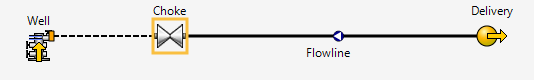
\includegraphics[scale=.9]{Fig/surface_equipment.PNG}
		\caption{Sơ đồ hệ thống thiết bị bề mặt}
		\label{fig:surface_equipment}
	\end{figure}
\newline
Trong phạm vi đồ án nhóm tác giả chỉ lựa chọn phân tích điểm nút tại đáy giếng ngay vị trí của lần bắn mở vỉa thứ nhất.
\newpage
	\begin{figure}[h]
		\centering
		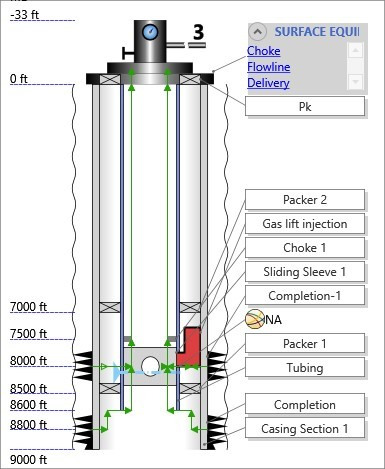
\includegraphics[scale=1.1]{Fig/1d_well_model.png}
		\caption{Mô hình một chiều của giếng}
		\label{fig:1d_well_model}
	\end{figure}
Ngoài ra nhóm tác giả còn đưa ra mô hình hai chiều của giếng theo các thông số khoan định hướng như Hình \ref{fig:2d_well_model}.
\newpage
	\begin{figure}[h]
		\centering
		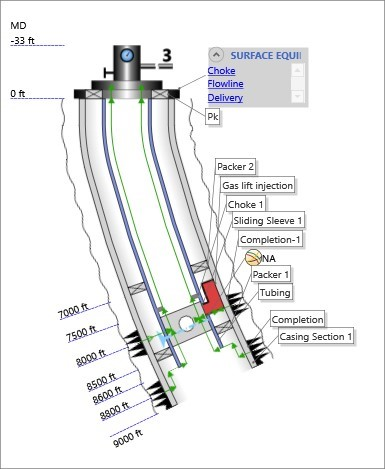
\includegraphics[scale=1.1]{Fig/2d_well_model.png}
		\caption{Mô hình hai chiều của giếng}
		\label{fig:2d_well_model}
	\end{figure}
Chiều sâu thực tế và độ dời đáy của giếng được thể hiện như trong đồ thị Hình \ref{fig:hd_directional_drilling}

\newpage
	\begin{figure}[h]
		\centering
		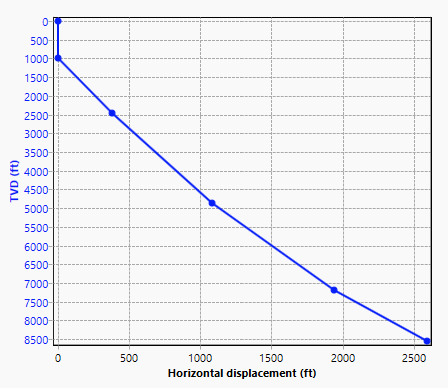
\includegraphics[scale=1.1]{Fig/hd_directional_drilling.PNG}
		\caption{Chiều sâu và độ dời đáy của giếng}
		\label{fig:hd_directional_drilling}
	\end{figure}

\section{Tính toán tối ưu hóa khai thác}
Điều kiện vận hành khai thác của giếng:
	\begin{itemize}
		\item Áp suất vỉa không đổi
		\item Lưu lượng khai thác trên 8000 STB/d
		\item Kích thước van tiết lưu 1 in.
	\end{itemize}
Dựa trên mô hình giếng và các điều kiện thực tế, nhóm tác giả chỉ đi vào phân tích các yếu tố chính là \textit{áp suất vỉa}, \textit{đường kính tubing}, \textit{chỉ số khai thác} và \textit{đường kính van tiết lưu}.

Với giai đoạn đầu khai thác áp suất vỉa còn chưa thay đổi, thay đổi kích thước van tiết lưu ta được các điểm vận hành như sau:
\newpage
	\begin{figure}[h]
		\centering
		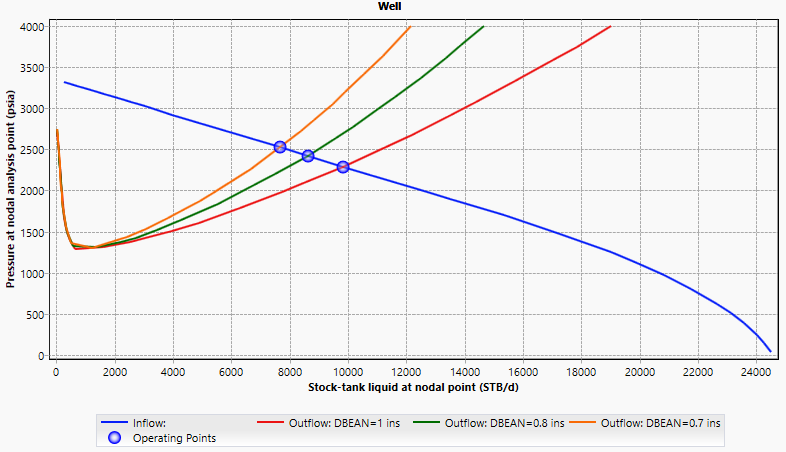
\includegraphics[scale=0.75]{Fig/Static_press_vs_choke.PNG}
		\caption{Điểm vận hành với các kích thước van tiết lưu khác nhau}
		\label{fig:Static_press_vs_choke}
	\end{figure}
Giá trị tại các điểm vận hành được thể hiện trong Bảng \ref{tab:static_press_vs_choke_result}.
\begin{table}[h]
\caption{Kết quả phân tích với áp suất vỉa không đổi}\label{tab:static_press_vs_choke_result}
\begin{tabularx}{\textwidth}{@{}XXX@{}}
\toprule
Điểm vận hành & Lưu lượng (STB/d) & Áp suất (psia) \\ \midrule
DBEAN=1 in    & 9844.934          & 2290.743       \\
DBEAN=0.8 in  & 8624.863          & 2422.37        \\
DBEAN=0.7 in  & 7780.741          & 2524.044       \\ \bottomrule
\end{tabularx}
\end{table}
\newline
Từ kết quả phân tích cho thấy trong giai đoạn áp suất vỉa chưa suy giảm, để đạt được lưu lượng khai thác như mong muốn đường kính van tiết lưu (DBEAN) có thể được đặt ở 0.8 in.
\newpage
Đối với sự thay đổi đường kính trong tubing, kết quả phân tích được thể hiện trong Hình \ref{fig:tubing_vs_static_press} và Bảng \ref{tab:tubing_vs_static_press_result}.
	\begin{figure}[h]
		\centering
		\includegraphics[scale=0.75]{Fig/tubing_vs_static_press.PNG}
		\caption{Điểm vận hành với các đường kính trong tubing khác nhau}
		\label{fig:tubing_vs_static_press}
	\end{figure}

\begin{table}[h]
\caption{Kết quả phân tích với đường kính trong tubing}\label{tab:tubing_vs_static_press_result}
\begin{tabularx}{\textwidth}{@{}XXX@{}}
\toprule
Điểm vận hành & Lưu lượng (STB/d) & Áp suất (psia) \\ \midrule
ID=3.985 in   & 9914.158          & 2283.796       \\
ID=3.476 in   & 8422.956          & 2434.761       \\
ID=2.992 in   & 6736.95           & 2604.85        \\ \bottomrule
\end{tabularx}
\end{table}
Khi thay đổi đường kính trong tubing, đường IPR không thay đổi nhiều. Tuy nhiên, đường OPR có sự thay đổi lớn, để đạt được lưu lượng khai thác lơn hơn 8000 STB/d đường kính trong tubing phù hợp là 3.476 in.
\newpage
Chỉ số khai thác thay đổi kết quả phân tích đạt được thể hiện như trong Hình \ref{fig:pi_vs_choke}.
	\begin{figure}[h]
		\centering
		\includegraphics[scale=0.75]{Fig/pi_vs_choke.PNG}
		\caption{Sự thay đổi chỉ số khai thác và đường kính van tiết lưu}
		\label{fig:pi_vs_choke}
	\end{figure}
\begin{table}[h]
\caption{Kết quả phân tích với sự thay đổi của chỉ số khai thác (DBEAN=1 in)}\label{tab:pi_vs_choke_result}
\begin{tabularx}{\textwidth}{@{}XXX@{}}
\toprule
Điểm vận hành          & Lưu lượng (STB/d) & Áp suất (psia) \\ \midrule
PI = 9.4 STB/(d.psi)  & 8423.103          & 2434.744       \\
PI = 8 STB/(d.psi)    & 7938.072          & 2341.531       \\
PI = 6 STB/(d.psi)    & 7006.33           & 2171.567       \\ \bottomrule
\end{tabularx}
\end{table}

Qua Bảng \ref{tab:pi_vs_choke_result} có thể thấy được khi chỉ số khai thác giảm xuống thấp, lưu lượng khai thác bắt đầu giảm. Lúc này, để có thể duy trì lưu lượng khai thác phải tăng đường kính van tiết lưu lớn nhất có thể (1 in) \nomenclature{PI}{Chỉ số khai thác}.

Khi áp suất vỉa bắt đầu suy giảm, vỉa không còn đủ năng lượng để có thể cho lưu lượng khai thác như mong muốn (đối với hệ thống khai thác đang sử dụng). Vì vậy, để duy trì lưu lượng khai thác cần phải thay đổi đường kính tubing. Kết quả phân tích được thể hiện như trong Hình \ref{fig:decrease_press_vs_tubing}.

	\begin{figure}[h]
		\centering
		\includegraphics[scale=0.75]{Fig/decrease_press_vs_tubing.PNG}
		\caption{Áp suất suy giảm với các kích thước tubing khác nhau}
		\label{fig:decrease_press_vs_tubing}
	\end{figure}

\begin{table}[h]
\caption{Kết quả phân tích với áp suất vỉa suy giảm}\label{tab:decrease_press_vs_tubing_result}
\begin{tabularx}{\textwidth}{@{}XXX@{}}
\toprule
Điểm vận hành & Lưu lượng (STB/d) & Áp suất (psia) \\ \midrule
ID=3.476 in   & 6353.533          & 2066.458       \\
ID=3.958 in   & 7490.071          & 1951.738       \\
ID=4.206 in   & 8004.196          & 1900.351       \\ \bottomrule
\end{tabularx}
\end{table}

Kết quả thực hiện phân tích như trong Bảng \ref{tab:decrease_press_vs_tubing_result} cho thấy khi áp suất vỉa bắt đầu suy giảm xuống dưới 3000 psi, để có thể duy trì lưu lượng khai thác cần tăng đường kính lên 4.206 in. Lúc này do áp suất vỉa xuống thấp làm cho áp suất qua van tiết lưu suy giảm theo, đồng thời chỉ có thể mở tối đa đường kính van tiết lưu lên 1 in, nên việc thay đổi đường kính van tiết lưu không còn được ưu tiên thực hiện. Kết quả được thể hiện như trong Hình \ref{fig:decrease_press_vs_choke_size}.
\newpage
	\begin{figure}[h]
		\centering
		\includegraphics[scale=0.75]{Fig/decrease_press_vs_choke_size.PNG}
		\caption{Thay đổi kích thước van tiết lưu theo sự suy giảm áp suất}
		\label{fig:decrease_press_vs_choke_size}
	\end{figure}

\begin{table}[h]
\caption{Kết quả phân tích suy giảm áp suất với kích thước van tiết lưu (DBEAN = 1 in)}\label{tab:decrease_press_vs_choke_size_result}
\begin{tabularx}{\textwidth}{@{}XXX@{}}
\toprule
Điểm vận hành                  & Lưu lượng (STB/d) & Áp suất (psia) \\ \midrule
PWSTATIC=3500 psia & 8089.64           & 2372.154       \\
PWSTATIC=3000 psia & 6359.535          & 2065.81        \\
PWSTATIC=2500 psia & 4526.497          & 1774.796       \\ \bottomrule
\end{tabularx}
\end{table}
Kết quả phân tích Bảng \ref{tab:decrease_press_vs_choke_size_result} cho thấy khi áp suất bắt đầu suy giảm kích thước van tiết lưu được mở ở mức tối đa cũng không thể duy trì lưu lượng khai thác như mong muốn.

\chapter*{\hspace*{4.4cm}KẾT LUẬN VÀ KIẾN NGHỊ}
\addcontentsline{toc}{chapter}{KẾT LUẬN VÀ KIẾN NGHỊ}
\section*{Kết luận}
\addcontentsline{toc}{section}{Kết luận}
Về cơ bản đồ án đã giải quyết được các vấn đề:
	\begin{itemize}
		\item Cơ sở lý thuyết của hệ thống khai thác và phân tích hệ thống khai thác bằng phân tích điểm nút
		\item Cơ sở xây dựng các đường đặc tính dòng vào và đường đặc tính dòng lên
		\item Bài toán cụ thể tối ưu hóa khai thác cho một giếng dầu bằng phần mềm PIPESIM với các điều kiện khai thác cho trước.
	\end{itemize}
\section*{Kiến nghị}
\addcontentsline{toc}{section}{Kiến nghị}
Bài toán thực tế của đồ án mới chỉ đi sâu về đặc tính kĩ thuật mà chưa đề cập đến hiệu quả kinh tế của phương pháp phân tích điểm nút. Do đó, nếu có điều kiện, đồ án nên tiếp tục được mở rộng về tính kinh tế để có thể thấy được toàn diện về phương pháp phân tích điểm nút.

\bibliographystyle{ieeetr}
\bibliography{ref}
\end{document}